\documentclass{sigplanconf}
%% ODER: format ==         = "\mathrel{==}"
%% ODER: format /=         = "\neq "
%
%
\makeatletter
\@ifundefined{lhs2tex.lhs2tex.sty.read}%
  {\@namedef{lhs2tex.lhs2tex.sty.read}{}%
   \newcommand\SkipToFmtEnd{}%
   \newcommand\EndFmtInput{}%
   \long\def\SkipToFmtEnd#1\EndFmtInput{}%
  }\SkipToFmtEnd

\newcommand\ReadOnlyOnce[1]{\@ifundefined{#1}{\@namedef{#1}{}}\SkipToFmtEnd}
\usepackage{amstext}
\usepackage{amssymb}
\usepackage{stmaryrd}
\DeclareFontFamily{OT1}{cmtex}{}
\DeclareFontShape{OT1}{cmtex}{m}{n}
  {<5><6><7><8>cmtex8
   <9>cmtex9
   <10><10.95><12><14.4><17.28><20.74><24.88>cmtex10}{}
\DeclareFontShape{OT1}{cmtex}{m}{it}
  {<-> ssub * cmtt/m/it}{}
\newcommand{\texfamily}{\fontfamily{cmtex}\selectfont}
\DeclareFontShape{OT1}{cmtt}{bx}{n}
  {<5><6><7><8>cmtt8
   <9>cmbtt9
   <10><10.95><12><14.4><17.28><20.74><24.88>cmbtt10}{}
\DeclareFontShape{OT1}{cmtex}{bx}{n}
  {<-> ssub * cmtt/bx/n}{}
\newcommand{\tex}[1]{\text{\texfamily#1}}	% NEU

\newcommand{\Sp}{\hskip.33334em\relax}


\newcommand{\Conid}[1]{\mathit{#1}}
\newcommand{\Varid}[1]{\mathit{#1}}
\newcommand{\anonymous}{\kern0.06em \vbox{\hrule\@width.5em}}
\newcommand{\plus}{\mathbin{+\!\!\!+}}
\newcommand{\bind}{\mathbin{>\!\!\!>\mkern-6.7mu=}}
\newcommand{\rbind}{\mathbin{=\mkern-6.7mu<\!\!\!<}}% suggested by Neil Mitchell
\newcommand{\sequ}{\mathbin{>\!\!\!>}}
\renewcommand{\leq}{\leqslant}
\renewcommand{\geq}{\geqslant}
\usepackage{polytable}

%mathindent has to be defined
\@ifundefined{mathindent}%
  {\newdimen\mathindent\mathindent\leftmargini}%
  {}%

\def\resethooks{%
  \global\let\SaveRestoreHook\empty
  \global\let\ColumnHook\empty}
\newcommand*{\savecolumns}[1][default]%
  {\g@addto@macro\SaveRestoreHook{\savecolumns[#1]}}
\newcommand*{\restorecolumns}[1][default]%
  {\g@addto@macro\SaveRestoreHook{\restorecolumns[#1]}}
\newcommand*{\aligncolumn}[2]%
  {\g@addto@macro\ColumnHook{\column{#1}{#2}}}

\resethooks

\newcommand{\onelinecommentchars}{\quad-{}- }
\newcommand{\commentbeginchars}{\enskip\{-}
\newcommand{\commentendchars}{-\}\enskip}

\newcommand{\visiblecomments}{%
  \let\onelinecomment=\onelinecommentchars
  \let\commentbegin=\commentbeginchars
  \let\commentend=\commentendchars}

\newcommand{\invisiblecomments}{%
  \let\onelinecomment=\empty
  \let\commentbegin=\empty
  \let\commentend=\empty}

\visiblecomments

\newlength{\blanklineskip}
\setlength{\blanklineskip}{0.66084ex}

\newcommand{\hsindent}[1]{\quad}% default is fixed indentation
\let\hspre\empty
\let\hspost\empty
\newcommand{\NB}{\textbf{NB}}
\newcommand{\Todo}[1]{$\langle$\textbf{To do:}~#1$\rangle$}

\EndFmtInput
\makeatother
%
%
%
%
%
%
% This package provides two environments suitable to take the place
% of hscode, called "plainhscode" and "arrayhscode". 
%
% The plain environment surrounds each code block by vertical space,
% and it uses \abovedisplayskip and \belowdisplayskip to get spacing
% similar to formulas. Note that if these dimensions are changed,
% the spacing around displayed math formulas changes as well.
% All code is indented using \leftskip.
%
% Changed 19.08.2004 to reflect changes in colorcode. Should work with
% CodeGroup.sty.
%
\ReadOnlyOnce{polycode.fmt}%
\makeatletter

\newcommand{\hsnewpar}[1]%
  {{\parskip=0pt\parindent=0pt\par\vskip #1\noindent}}

% can be used, for instance, to redefine the code size, by setting the
% command to \small or something alike
\newcommand{\hscodestyle}{}

% The command \sethscode can be used to switch the code formatting
% behaviour by mapping the hscode environment in the subst directive
% to a new LaTeX environment.

\newcommand{\sethscode}[1]%
  {\expandafter\let\expandafter\hscode\csname #1\endcsname
   \expandafter\let\expandafter\endhscode\csname end#1\endcsname}

% "compatibility" mode restores the non-polycode.fmt layout.

\newenvironment{compathscode}%
  {\par\noindent
   \advance\leftskip\mathindent
   \hscodestyle
   \let\\=\@normalcr
   \let\hspre\(\let\hspost\)%
   \pboxed}%
  {\endpboxed\)%
   \par\noindent
   \ignorespacesafterend}

\newcommand{\compaths}{\sethscode{compathscode}}

% "plain" mode is the proposed default.
% It should now work with \centering.
% This required some changes. The old version
% is still available for reference as oldplainhscode.

\newenvironment{plainhscode}%
  {\hsnewpar\abovedisplayskip
   \advance\leftskip\mathindent
   \hscodestyle
   \let\hspre\(\let\hspost\)%
   \pboxed}%
  {\endpboxed%
   \hsnewpar\belowdisplayskip
   \ignorespacesafterend}

\newenvironment{oldplainhscode}%
  {\hsnewpar\abovedisplayskip
   \advance\leftskip\mathindent
   \hscodestyle
   \let\\=\@normalcr
   \(\pboxed}%
  {\endpboxed\)%
   \hsnewpar\belowdisplayskip
   \ignorespacesafterend}

% Here, we make plainhscode the default environment.

\newcommand{\plainhs}{\sethscode{plainhscode}}
\newcommand{\oldplainhs}{\sethscode{oldplainhscode}}
\plainhs

% The arrayhscode is like plain, but makes use of polytable's
% parray environment which disallows page breaks in code blocks.

\newenvironment{arrayhscode}%
  {\hsnewpar\abovedisplayskip
   \advance\leftskip\mathindent
   \hscodestyle
   \let\\=\@normalcr
   \(\parray}%
  {\endparray\)%
   \hsnewpar\belowdisplayskip
   \ignorespacesafterend}

\newcommand{\arrayhs}{\sethscode{arrayhscode}}

% The mathhscode environment also makes use of polytable's parray 
% environment. It is supposed to be used only inside math mode 
% (I used it to typeset the type rules in my thesis).

\newenvironment{mathhscode}%
  {\parray}{\endparray}

\newcommand{\mathhs}{\sethscode{mathhscode}}

% texths is similar to mathhs, but works in text mode.

\newenvironment{texthscode}%
  {\(\parray}{\endparray\)}

\newcommand{\texths}{\sethscode{texthscode}}

% The framed environment places code in a framed box.

\def\codeframewidth{\arrayrulewidth}
\RequirePackage{calc}

\newenvironment{framedhscode}%
  {\parskip=\abovedisplayskip\par\noindent
   \hscodestyle
   \arrayrulewidth=\codeframewidth
   \tabular{@{}|p{\linewidth-2\arraycolsep-2\arrayrulewidth-2pt}|@{}}%
   \hline\framedhslinecorrect\\{-1.5ex}%
   \let\endoflinesave=\\
   \let\\=\@normalcr
   \(\pboxed}%
  {\endpboxed\)%
   \framedhslinecorrect\endoflinesave{.5ex}\hline
   \endtabular
   \parskip=\belowdisplayskip\par\noindent
   \ignorespacesafterend}

\newcommand{\framedhslinecorrect}[2]%
  {#1[#2]}

\newcommand{\framedhs}{\sethscode{framedhscode}}

% The inlinehscode environment is an experimental environment
% that can be used to typeset displayed code inline.

\newenvironment{inlinehscode}%
  {\(\def\column##1##2{}%
   \let\>\undefined\let\<\undefined\let\\\undefined
   \newcommand\>[1][]{}\newcommand\<[1][]{}\newcommand\\[1][]{}%
   \def\fromto##1##2##3{##3}%
   \def\nextline{}}{\) }%

\newcommand{\inlinehs}{\sethscode{inlinehscode}}

% The joincode environment is a separate environment that
% can be used to surround and thereby connect multiple code
% blocks.

\newenvironment{joincode}%
  {\let\orighscode=\hscode
   \let\origendhscode=\endhscode
   \def\endhscode{\def\hscode{\endgroup\def\@currenvir{hscode}\\}\begingroup}
   %\let\SaveRestoreHook=\empty
   %\let\ColumnHook=\empty
   %\let\resethooks=\empty
   \orighscode\def\hscode{\endgroup\def\@currenvir{hscode}}}%
  {\origendhscode
   \global\let\hscode=\orighscode
   \global\let\endhscode=\origendhscode}%

\makeatother
\EndFmtInput
%

\usepackage{array, amssymb, amsthm, amsmath, mathpartir,thmtools}
\usepackage[usenames,dvipsnames]{color}
\usepackage{tikz}
\newcommand{\Red}[1]{{\color{red} #1}}
\newcommand{\todo}[2]{\Red{\textbf{TODO[}#1\textbf{]:} #2}} % chktex 9
%\newcommand{\todo}[2]{}
\newcommand{\cut}[1]{}
\newcommand{\alphacondition}[1]{{\color{green}Condition for $\alpha$: #1}}

\usepackage{wrapfig}
\usepackage[square,numbers,sort&compress]{natbib}

\newcommand{\tocite}[1]{\Red{\cite{#1}}}
\newcommand{\toref}[1]{\Red{\ref{#1}}}

\usepackage{float}
\newfloat{listing}{htbp}{lop} \floatname{listing}{Listing}

\declaretheorem{theorem}
\declaretheorem[name=Lemma]{lemma}
\declaretheorem[name=Corollary]{corollary}
\declaretheorem[name=Proposition]{proposition}
% thmstyle: definition
\declaretheorem[name=Definition, style=definition]{definition}
\declaretheorem[name=Example, style=definition]{example}
% thmstyle: remark
\declaretheorem[name=Proof sketch, style=remark]{proofsketch}



\begin{document}




% label operation related:
\newcommand{\flows}{\sqsubseteq}
\newcommand{\lub}{\sqcup}
\newcommand{\glb}{\sqcap}



\newcommand{\ifc}[1]{\ensuremath{{\color{blue} #1}}}
\newcommand{\lcurr}{\ensuremath{\ifc{l_{\textrm{cur}}}}}

%%%%%%%%%%%%%%%%%%%%%%%%%%%%%%%%%%%%%%%%%%%%%%%%%%%%%%%%%%%%%%%%%%%
%% state, eval ctx, expression












%%%%%%%%%%%%%%%%%%%%%%%%%%%%%%%%%%%%%%%%%%%%%%%%%%%%%%%%%%%%%%%%%%%
%% IFC state, eval ctx, expression























%%%%%%%%%%%%%%%%%%%%%%%%%%%%%%%%%%%%%%%%%%%%%%%%%%%%%%%%%%%%%%%%%%%
%% TARGET state, eval ctx, expression
\newcommand{\tar}[1]{\ensuremath{\mathbf{\color{red} #1}}}








%formtt tty'
%formtt tty''
%formtt ttyi = tty"_"i
%formtt ttyi' = tty'"_"i
%formtt ttyi'' = tty''"_"i
%formtt tty1
%formtt tty2
%formtt tty3
%formtt tty1'
%formtt tty2'
%formtt tty3'
%formtt tty1''
%formtt tty2''
%formtt tty3''


%%%%%%%%%%%%%%%%%%%%%%%%%%%%%%%%%%%%%%%%%%%%%%%%%%%%%%%%%%%%%%%%%%%

%% language
\newcommand{\Coloneqq}{::=} % txfonts

%% misc
\newcommand{\dom}[1]{\ensuremath{{\textrm{dom}} #1}}
\newcommand{\fresh}[1]{\ensuremath{\textrm{fresh}(#1)}}









%%%%%%%%%%%%%%%%%%%%%%%%%%%%%%%%%%%%%%%%%%%%%%%%%%%%%%%%%%%%%%%%%%%
%% Combined state, eval ctx, expression


% Going to use S




%%%%%
%% LANGUAGES



%%%%%
%% From concrete

% ----------
%% \conferenceinfo{ICFP'14,} {September 1--3, 2013, Gothenburg, Sweden.}
%% \CopyrightYear{2014}
%% \copyrightdata{XXX-X-XXXX-XXXX-X/XX/XX}
% ----------

\title{
Just Add IFC! A General Approach to Retrofitting Languages with Dynamic Information Flow Control
}
%   Generic, Efficient, Coarse-grained Information Flow Control
%   IFC For Me
%   Who knew adding IFC could be us easy?
%   Language-polymorphic schemes of dynamic information flow control
%   Target language and IFC language: shake to mix
%   1. Target language, 2. IFC language, 3. ... 4. Profit!!!
%   Just add IFC

\authorinfo{
  Stefan Heule \and
  Deian Stefan \and
  Edward Z. Yang \and
  John C. Mitchell \and
  Alejandro Russo
}{Stanford University, Chalmers University}{
\text{\tt \char123{}sheule\char44{}deian\char44{}ezyang\char44{}mitchell\char125{}\char64{}cs\char46{}stanford\char46{}edu}, \text{\tt russo\char64{}chalmers\char46{}se}
}

\maketitle

\begin{abstract}
Many important security problems in JavaScript, such as browser
extension security, untrusted JavaScript libraries and safe
integration of mutually distrustful websites (mash-ups), may be
effectively addressed using an efficient implementation of information
flow control (IFC).  Unfortunately existing fine-grained approaches to
JavaScript IFC require modifications to the language semantics, a
non-goal for browser applications.  In this work we take the ideas of
coarse-grained dynamic IFC to the limit and provide the theoretical
foundation for a language-based approach that can be applied to any
programming language for which external effects can be controlled.  We
then apply this formalism to JavaScript, in the context of Node.js and
Firefox, and show how it generalizes to the C programmings language.  Our methodology offers
design principles for the construction of information flow control
systems when isolation can easily be achieved, as well as
compositional proofs for optimized concrete implementations of these
systems, by relating them to their fully isolated variants.
\end{abstract}

\section{Introduction}
\label{sec:intro}
%   \Red{DM had some very good comments on how to make this sound less
%     like a pitch for LIO. Outline for something more compelling (not
%     necessarily in this order):
%   \begin{itemize}
%     \item Motivate IFC
%     \item Coarse grained IFC is easy
%     \item Coarse grained IFC is sufficient (vs. fine grained); do by citation
%     \item We have the right API and it's language-agnostic; proof is also language independent
%     \item You can ``drop it in''
%   \end{itemize}
%   }

Modern web content is rendered using a potentially large number of
different components with differing provenance.
Disparate and untrusting components may arise from browser
extensions (whose JavaScript code runs alongside website
code), web applications (with possibly untrusted third-party
libraries), and mashups (which combine code and data from
websites that may not even be aware of each other's existence.)
While just-in-time combination of untrusting components
offers great flexibility, it also poses complex security challenges.
In particular, maintaining data privacy in the face of malicious
extensions, libraries, and mashup components has been difficult,
and in general effectively impossible.

Information flow control (IFC) is a promising technique
that provides security
by tracking the flow of sensitive data through a system.
Untrusted code is confined so that it cannot exfiltrate data, except as
per an information flow policy.  Significant research has been devoted to
adding various forms of IFC to different kinds of programming languages
and systems.  In the context of the web, however, there is a strong
motivation to preserve JavaScript's semantics while retrofitting it with dynamic information
flow control.

One approach to information flow control is fine-grained tracking,
which offers great flexibility.
However, these systems
require deep integration with the programming language and modify
the semantics in non-trivial ways.  This makes fine-grained systems
less suitable in contexts where preserving an existing language
is important.
%
Moreover, the task of adding fine-grained IFC even to a simple language is
non-trivial~\cite{hritcu2013testing}; when considering a real-world language,
such as JavaScript, this challenge becomes almost insurmountable.

In the alternative \textit{coarse-grained} approach to IFC,
a system is divided into relatively coarse computational units,
each with a single label dictating its security policy.
Only
communication between isolated computational units must be tracked.
%A recent system named SWAPI~\cite{swapi} adds IFC to the
%browser by identifying \emph{web workers} as an existing computational
%unit.  Communication between workers is mediated using
%IFC to ensure non-interference, preventing sensitive workers from
%influencing the computation of less sensitive workers.
This coarse-grained approach provides a number of advantages:
(1) minimal changes to an
existing programming language when adding IFC, which (2) allows
the reuse of existing programs.  Furthermore, (3)
reduced runtime overhead because checks need only
be performed at isolation boundaries, compared to fine-grained
systems were the runtime overhead can be impractical~\cite{JSFlow}.
Finally, (4) associating
a single security label with the entire computational unit simplifies
understanding and reasoning about the correctness of the
system, without information flow reasoning about the
technical details of the semantics of the programming language.

In this paper, we take coarse-grained labeling~\cite{Zeldovich:2006,
lio} to its logical extreme: an information flow control system should
be thought of as multiple instances of completely isolated language
runtimes or \emph{tasks}, with information flow control applied to
inter-task communication.  We describe a formal system in which an IFC
system can be designed once and then applied to any programming language
which has control over external effects (e.g., JavaScript or C with
access to hardware privilege separation).  We formalize this system
using an approach by
Matthews-Findler~\cite{Matthews:2007:OSM:1190216.1190220} for combining
operational semantics and prove non-interference guarantees
that are independent of the choice of specific target language.

There are a number of points that distinguish this setting from
previous coarse-grained IFC systems:
%
First, even though the underlying semantic model involves communicating
tasks, these tasks can be coordinated together in ways that simulate
traditional features in monolithic languages.  In fact, simulating
features in this way is a very useful \emph{design tool} for discovering
what variants of the features are permissible and which are not.
%
Second, although completely separate tasks are semantically easy to
reason about, real-world implementations often blur the lines between
tasks in the name of efficiency.
Characterizing what optimizations are permissible is subtle, since
removing transitions from the operational semantics of a language can
break non-interference.  We partially address this issue
by characterizing isomorphisms between the operational semantics of our
defined language and a concrete implementation, showing that if this
relationship holds, then non-interference in the abstract specification
carries over to the concrete implementation.

Our contributions can be summarized as follows:
\begin{itemize}
  \item We give formal semantics for a core coarse-grained
  dynamic information flow control language free of non-IFC constructs.
  We then show how a large class of target languages can be combined
  with this IFC language and prove that the result provides
  non-interference. (Section~\ref{sec:retrofit})
  \item We provide a proof technique to show the non-interference
  of a concrete semantics for a potentially optimized IFC language
  by means of an isomorphism, and show a class of restrictions on
  the IFC language that preserves non-interference. (Section~\ref{sec:formal}
  and~\ref{sec:concrete})
  \item We have implemented an IFC system based on these semantics
  for Node.js, and we connect our formalism to another implementation
  based on this work
  for client-side JavaScript in Gecko~\cite{swapi}.
  Furthermore, we outline an implementation for the C programming
  language.
  (Section~\ref{sec:real})
%  \item We show how to extend the Matthews-Findler method from just
%  languages that are not simply expressions evaluating to values,
%  but may be collections of threads executing nondeterministically.
  \item We describe ways to enrich the core IFC language with
  more advanced concepts such as labeled values, labeled references, or a
  notion of clearance. (Section~\ref{sec:extensions})
\end{itemize}

\cut{

(Something about the importance of IFC).

One barrier to the adoption of information flow control has been the
fact that it often incurs a large performance cost.  This usually stems
from the fact that most existing programming languages do not have
facilities for enforcing isolation.  Thus information flow control
checks must be applied at a very fine-grained level, e.g.\ all values in
the system must be labeled, resulting in large overhead for ordinary
operations.

Motivated by these problems, there has been increasing interest in
coarse-grained IFC systems, which trade-off precision for reduced
overhead.  These systems are characterized by floating label associated
with a thread of execution, so that access to labeled data taints the
entire thread, solving the problem of flow-sensitivity.  Typically,
these systems require strong isolation between threads, which previously
has been enforced by the type system. (LIO)  This has made this method
difficult to apply to languages which are unable to statically enforce
such strong isolation.

In this paper, we describe a simple but general methodology for using
isolation of \emph{execution contexts}, e.g.\ an instance of the
JavaScript engine, in order to add information-flow control to an
existing language.  This is a very practical approach, as there are many
languages which have built-in capabilities for strong isolation by
forking an execution context (i.e. Web Workers).  To validate this
methodology, we describe its application to Haskell (LIO), to JavaScript
(Browbound), to C (HipStar) and to Java (Aeolis).  The essential idea is
to combine the formal models of the source language and a minimal IFC
language, using the embedding technique described in Matthews and
Findler '07.

Our contributions are as follows:

\begin{itemize}
    \item We define a minimal IFC language which describes the essence
        of coarse-grained information flow control.

    \item We describe how to combine this IFC language with an existing
        source language in the style of Matthews-Findler, with a twist:
        there are arbitrarily many copies of the source language, which
        do not share execution contexts.  Mediating between these languages
        requires serialization of some sort (we make this notion precise
        in our paper), making our combined system a distributed one.

    \item We carry out this methodology on four existing languages, and
        show its adequacy with respect to systems that were specialized
        for these languages.  In particular, our definitions are general
        enough to enable relaxed isolation when the source language is
        able to give stronger static guarantees.

    \item We show how to extend the Matthews-Findler method from just
        languages that are not simply expressions evaluating to values,
        but may be collections of threads executing nondeterministically.
\end{itemize}

The organization of the paper is as follows: first, we describe how to
add information flow control to JavaScript, showing the general outline of
our procedure. Next, we describe the procedure in generality.  Finally, we
apply the procedure to a number of systems.
}


\section{Retrofitting languages with IFC}
\label{sec:retrofit}

Our overall plan will be to take a \textbf{{\color{red} target language}} with a formal
operational semantics and combine it with an \textit{{\color{blue} information
flow control language}}.  For concreteness, we use a simple, untyped,
ML-like language with mutable references as our target language.
However, our technique will be indifferent to the actual target language
chosen: it need only be prepared for interoperability by being expressed
in the style of Matthews and
Findler~\cite{Matthews:2007:OSM:1190216.1190220}.  This procedure will
equip the target language with primitives for implementing dynamic
information control in the style of LIO~\cite{lio}, which we will
describe in more detail shortly.

We have typeset nonterminals of the target language using \textbf{{\color{red}
bold font}} while the nonterminals of the IFC language have been typeset
with \textit{{\color{blue} italic font}}.  Readers are encouraged to view
a color copy of this paper, where target language nonterminals are colored red
while IFC language nonterminals are colored blue.

\subsection{Target language: Mini-ML}

In Figure~\ref{fig:ml}, we give a simple, untyped ML-like language with
mutable references and errors, prepared for combination with an
information flow control language.  The presentation is standard, but it
is worth paying some attention to the Felleisen-Hieb reduction
semantics~\cite{Felleisen:1992:RRS:136293.136297} used to define the
operational semantics of the system.  Our language defines an evaluation
context \ensuremath{\tar{E}}; however, the evaluation rules have been expressed in terms
of a different evaluation context $\mathcal{E}_{\tar{\Sigma}}$.  To
derive the usual operational semantics for this language, the evaluation
context merely needs to be defined as \ensuremath{\mathcal{E}_{\tar{\Sigma}}\left[\tar{e}\right]\triangleq{}\tar{\Sigma},\tar{E}\;[\mskip1.5mu \tar{e}\mskip1.5mu]}.
However, when we combine this language with an IFC language, we must
reinterpret the meaning of this evaluation context.
In general, we require that a target language be expressed in terms
of some global machine state \ensuremath{\tar{\Sigma}}, some evaluation context \ensuremath{\tar{E}},
some expressions \ensuremath{\tar{e}}, some set of values \ensuremath{\tar{v}} and a reduction
relations on full configurations $\ensuremath{\tar{\Sigma}} \times \ensuremath{\tar{E}} \times \ensuremath{\tar{e}}$.

\begin{figure}
\begin{hscode}\SaveRestoreHook
\column{B}{@{}>{\hspre}l<{\hspost}@{}}%
\column{6}{@{}>{\hspre}l<{\hspost}@{}}%
\column{8}{@{}>{\hspre}l<{\hspost}@{}}%
\column{22}{@{}>{\hspre}l<{\hspost}@{}}%
\column{40}{@{}>{\hspre}l<{\hspost}@{}}%
\column{47}{@{}>{\hspre}l<{\hspost}@{}}%
\column{E}{@{}>{\hspre}l<{\hspost}@{}}%
\>[B]{}\tar{v}{}\<[6]%
\>[6]{}\Coloneqq\lambda \tar{x}.\tar{e}\mid \mathbf{true}\mid \mathbf{false}\mid \tar{a}{}\<[E]%
\\
\>[B]{}\tar{e}{}\<[6]%
\>[6]{}\Coloneqq\tar{v}\mid \tar{x}\mid \tar{e}\;\tar{e}\mid \mathbf{if}\;\tar{e}\;\mathbf{then}\;\tar{e}\;\mathbf{else}\;\tar{e}\mid \mathbf{ref}\;\tar{e}\mid \mathbin{!}\tar{e}\mid \tar{e}\mathbin{:=}\tar{e}{}\<[E]%
\\
\>[B]{}\tar{E}{}\<[6]%
\>[6]{}\Coloneqq\tar{[\cdot ]_T}\mid \tar{E}\;\tar{e}\mid \tar{v}\;\tar{E}\mid \mathbf{if}\;\tar{E}\;\mathbf{then}\;\tar{e}\;\mathbf{else}\;\tar{e}{}\<[E]%
\\
\>[6]{}\hsindent{2}{}\<[8]%
\>[8]{}\mid \mathbf{ref}\;\tar{E}\mid \mathbin{!}\tar{E}\mid \tar{E}\mathbin{:=}\tar{e}\mid \tar{v}\mathbin{:=}\tar{E}{}\<[E]%
\\[\blanklineskip]%
\>[B]{}\tar{e}_{1};\tar{e}_{2}{}\<[22]%
\>[22]{}\triangleq{}(\lambda \tar{x}.\tar{e}_{2})\;\tar{e}_{1}\;{}\<[40]%
\>[40]{}\mathbf{where}\;{}\<[47]%
\>[47]{}\tar{x}\;\not\in\;\mathcal{FV}\;(\tar{e}_{2}){}\<[E]%
\\
\>[B]{}\mathbf{let}\;\tar{x}\mathrel{=}\tar{e}_{1}\;\mathbf{in}\;\tar{e}_{2}{}\<[22]%
\>[22]{}\triangleq{}(\lambda \tar{x}.\tar{e}_{2})\;\tar{e}_{1}{}\<[E]%
\ColumnHook
\end{hscode}\resethooks

\begin{mathpar}

\and
\inferrule[T-app]
{ } {\ensuremath{\mathcal{E}_{\tar{\Sigma}}\left[(\lambda \Varid{x}.\tar{e})\;\tar{v}\right]\rightarrow\mathcal{E}_{\tar{\Sigma}}\left[\{\mskip1.5mu \tar{v}\mathbin{/}\Varid{x}\mskip1.5mu\}\;\tar{e}\right]}}

\and
\inferrule[T-ifTrue]
{ } {\ensuremath{\mathcal{E}_{\tar{\Sigma}}\left[\;\mathbf{if}\;\mathbf{true}\;\mathbf{then}\;\tar{e}_{1}\;\mathbf{else}\;\tar{e}_{2}\right]\rightarrow\mathcal{E}_{\tar{\Sigma}}\left[\tar{e}_{1}\right]}}

\and
\inferrule[T-ifFalse]
{ } {\ensuremath{\mathcal{E}_{\tar{\Sigma}}\left[\;\mathbf{if}\;\mathbf{false}\;\mathbf{then}\;\tar{e}_{1}\;\mathbf{else}\;\tar{e}_{2}\right]\rightarrow\mathcal{E}_{\tar{\Sigma}}\left[\tar{e}_{2}\right]}}

\and
\inferrule[T-ref]
{ \ensuremath{\textrm{fresh}(\tar{a})} }
{\ensuremath{\mathcal{E}_{\tar{\Sigma}}\left[\mathbf{ref}\;\tar{v}\right]\rightarrow\mathcal{E}_{\tar{\Sigma}\left[\tar{a}\mapsto{}\tar{v}\right]}\left[\tar{a}\right]}}

\and
\inferrule[T-deref]
{ \ensuremath{(\tar{a},\tar{v})\;\mathbf{in}\;\tar{\Sigma}} }
{\ensuremath{\mathcal{E}_{\tar{\Sigma}}\left[\mathbin{!}\tar{a}\right]\rightarrow\mathcal{E}_{\tar{\Sigma}}\left[\tar{v}\right]}}

\and
\inferrule[T-ass]
{ }
{\ensuremath{\mathcal{E}_{\tar{\Sigma}}\left[\tar{a}\mathbin{:=}\tar{v}\right]\rightarrow\mathcal{E}_{\tar{\Sigma}\left[\tar{a}\mapsto{}\tar{v}\right]}\left[\tar{v}\right]}}

%\and
%\inferrule[T-fail]
%{| conf tS ( tE [ fail ] ) -> conf tS fail |}
\end{mathpar}

\caption{Simple ML-like language \ensuremath{\Red{\lambda_{\text{ML}}}}}
\label{fig:ml}
\end{figure}

\subsection{IFC language}

Information flow control seeks to enforce a security policy known as
\emph{non-interference}: public results must not depend on secret inputs.
Modern, dynamic IFC systems usually achieve this by associating a \emph{label}
with data, which encodes a policy of whether or not data tagged with one
label can flow to another label (written as \ensuremath{\flows}).
Since our embedding is agnostic
to the choice of labeling scheme, we simply represent labels with the metavariable
$l$, but do not discuss them in more detail.

In Figure~\ref{fig:ifc}, we give the syntax and \emph{single-threaded}
evaluation rules for a minimal information-flow control language.  The
evaluation context $\mathcal{E}_{\ifc{\Sigma}}$ represents the context
of the current task which is running, including on the right-hand side
the current label $l$ (which protects the program counter of the task)
and the task ID $i$.

Ordinarily, information flow control languages are defined by directly
stating a base language plus information flow control operators.  In
contrast, our language is purposely minimal: it does not have sequencing
operations, control flow, or other constructs.  However, it contains
support for the following core information flow control features:

\begin{itemize}
    \item First-class labels, with label values $l$ as well as operations for computing on
labels (\ensuremath{\flows}, \ensuremath{\lub} and \ensuremath{\glb}),
    \item operations for inspecting (\textbf{getLabel}) and modifying (\textbf{setLabel}) the current label of the task (a task can only increase its label, and not decrease it),
    \item operations for non-blocking inter-task communication (\textbf{send} and \textbf{recv}),
        which interact with the global store of per-task message queues \ensuremath{\ifc{\Sigma}}, and
    \item a sandboxing operation allowing to spawn new
    isolated tasks, which will be described in more detail in the
    next section.
\end{itemize}

The form of \textbf{send}/\textbf{recv} are \Red{inspired by methods of inter-worker communication
in web browser APIs} \Red{cite}, however in Section~\ref{sec:extensions} we
discuss other possible choices for information flow control aware communication
primitives.  Their rules are different from non-IFC systems
and worth commenting on: when a task places
a message on the message queue of receiving task, it also labels that
message with a label \ensuremath{\ifc{\Varid{l}}'} (which must be above the tasks current label \ensuremath{\ifc{\Varid{l}}})
When the recipient reads out messages from its queue,
messages whose labels do not
flow to \ensuremath{\ifc{\Varid{l}}} are filtered out (denoted by \ensuremath{\ifc{\Theta}\preceq\ifc{\Varid{l}}}).
Specifically, if \ensuremath{\ifc{\Theta}} is the empty list \ensuremath{\epsilon}, the
function is simply the identity function, i.e.,
\ensuremath{\epsilon\preceq\ifc{\Varid{l}}\mathrel{=}\epsilon}; otherwise:
\[
\ensuremath{(\ifc{\Varid{l}}',\ifc{\Varid{i}},\ifc{\Varid{e}}),\ifc{\Theta}\preceq\ifc{\Varid{l}}} = \left\{
\begin{array}{l l}
\ensuremath{(\ifc{\Varid{l}}',\ifc{\Varid{i}},\ifc{\Varid{e}}),\ifc{\Theta}\preceq\ifc{\Varid{l}}} & \quad \text{if \ensuremath{\ifc{\Varid{l}}'\;\flows\;\ifc{\Varid{l}}}}\\
\ensuremath{\ifc{\Theta}\preceq\ifc{\Varid{l}}} & \quad \text{otherwise}
\end{array} \right.
\]
This ensures that tasks cannot receive messages that are more secret
than their current label would allow.

%   \begin{figure}
%   Typing judgment: $|tyrule tG tS te tty|$
%   \begin{mathpar}
%   \inferrule[T-ty-address]
%   {}
%   {| tyrule tG tS a (ref (tyLookup tS a)) |}
%   \end{mathpar}

%   \caption{Selected typing rules for ML-like language}
%   \label{fig:ml-typing}
%   \end{figure}

\begin{figure}
\begin{hscode}\SaveRestoreHook
\column{B}{@{}>{\hspre}l<{\hspost}@{}}%
\column{6}{@{}>{\hspre}c<{\hspost}@{}}%
\column{6E}{@{}l@{}}%
\column{8}{@{}>{\hspre}c<{\hspost}@{}}%
\column{8E}{@{}l@{}}%
\column{11}{@{}>{\hspre}l<{\hspost}@{}}%
\column{E}{@{}>{\hspre}l<{\hspost}@{}}%
\>[B]{}\otimes{}\<[6]%
\>[6]{}\Coloneqq{}\<[6E]%
\>[11]{}\flows\mid \lub\mid \glb{}\<[E]%
\\
\>[B]{}\ifc{\Varid{v}}{}\<[6]%
\>[6]{}\Coloneqq{}\<[6E]%
\>[11]{}\ifc{\Varid{i}}\mid \ifc{\Varid{l}}\mid \mathbf{true}\mid \mathbf{false}\mid \langle\rangle{}\<[E]%
\\
\>[B]{}\ifc{\Varid{e}}{}\<[6]%
\>[6]{}\Coloneqq{}\<[6E]%
\>[11]{}\ifc{\Varid{v}}\mid \ifc{\Varid{x}}\mid \ifc{\Varid{e}}\;\otimes\;\ifc{\Varid{e}}\mid \mathbf{getLabel}\mid \mathbf{setLabel}\;\ifc{\Varid{e}}{}\<[E]%
\\
\>[6]{}\hsindent{2}{}\<[8]%
\>[8]{}\mid {}\<[8E]%
\>[11]{}\mathbf{sandbox}\;\ifc{\Varid{e}}\mid \mathbf{send}\;\ifc{\Varid{e}}\;\ifc{\Varid{e}}\;\ifc{\Varid{e}}\mid \ifc{\Varid{x}}_{1},\ifc{\Varid{x}}_{2}\Leftarrow\mathbf{recv}.\ifc{\Varid{e}}\;\ifc{\Varid{e}}{}\<[E]%
\\
\>[B]{}\ifc{E}{}\<[6]%
\>[6]{}\Coloneqq{}\<[6E]%
\>[11]{}\ifc{[\cdot ]_I}\mid \ifc{E}\;\otimes\;\ifc{\Varid{e}}\mid \ifc{\Varid{v}}\;\otimes\;\ifc{E}\mid \mathbf{setLabel}\;\ifc{E}\mid \mathbf{sandbox}\;\ifc{E}{}\<[E]%
\\
\>[6]{}\hsindent{2}{}\<[8]%
\>[8]{}\mid {}\<[8E]%
\>[11]{}\mathbf{send}\;\ifc{E}\;\ifc{\Varid{e}}\;\ifc{\Varid{e}}\mid \mathbf{send}\;\ifc{\Varid{v}}\;\ifc{E}\;\ifc{\Varid{e}}\mid \mathbf{send}\;\ifc{\Varid{v}}\;\ifc{\Varid{v}}\;\ifc{E}{}\<[E]%
\\
\>[6]{}\hsindent{2}{}\<[8]%
\>[8]{}\mid {}\<[8E]%
\>[11]{}\ifc{\Varid{x}}_{1},\ifc{\Varid{x}}_{2}\Leftarrow\mathbf{recv}.\ifc{\Varid{e}}\;\ifc{\Varid{e}}{}\<[E]%
\\
\>[B]{}\ifc{\theta}{}\<[6]%
\>[6]{}\Coloneqq{}\<[6E]%
\>[11]{}(\ifc{\Varid{l}},\ifc{\Varid{i}}\;\ifc{\Varid{e}}){}\<[E]%
\\
\>[B]{}\ifc{\Theta}{}\<[6]%
\>[6]{}\Coloneqq{}\<[6E]%
\>[11]{}\epsilon\mid \ifc{\theta},\ifc{\Theta}{}\<[E]%
\\
\>[B]{}\ifc{\Sigma}{}\<[6]%
\>[6]{}\Coloneqq{}\<[6E]%
\>[11]{}\emptyset\mid \ifc{\Sigma}\left[\ifc{\Varid{i}}\mapsto{}\ifc{\Theta}\right]{}\<[E]%
\ColumnHook
\end{hscode}\resethooks

\begin{mathpar}

\and
\inferrule[I-getLabel]
{ }
{\ensuremath{\mathcal{E}_{\ifc{\Sigma}}\left[\mathbf{getLabel}\right]^{\ifc{\Varid{i}}}_{\ifc{\Varid{l}}}\rightarrow\mathcal{E}_{\ifc{\Sigma}}\left[\ifc{\Varid{l}}\right]^{\ifc{\Varid{i}}}_{\ifc{\Varid{l}}}}}

\and
\inferrule[I-setLabel]
{ \ensuremath{\ifc{\Varid{l}}\;\flows\;\ifc{\Varid{l}}'} }
{\ensuremath{\mathcal{E}_{\ifc{\Sigma}}\left[\mathbf{setLabel}\;\ifc{\Varid{l}}'\right]^{\ifc{\Varid{i}}}_{\ifc{\Varid{l}}}\rightarrow\mathcal{E}_{\ifc{\Sigma}}\left[\langle\rangle\right]^{\ifc{\Varid{i}}}_{\ifc{\Varid{l}}'}}}
%{|fresh (id')|}

\and
\inferrule[I-send]
{
\ensuremath{\ifc{\Varid{l}}\;\flows\;\ifc{\Varid{l}}'}\\
\ensuremath{\ifc{\Sigma}\;(\ifc{\Varid{i}}')\mathrel{=}\ifc{\Theta}}\\
\ensuremath{\ifc{\Sigma}'\mathrel{=}\ifc{\Sigma}\left[\ifc{\Varid{i}}'\mapsto{}(\ifc{\Varid{l}}',\ifc{\Varid{i}},\ifc{\Varid{e}}),\ifc{\Theta}\right]}
}
{\ensuremath{\mathcal{E}_{\ifc{\Sigma}}\left[\mathbf{send}\;\ifc{\Varid{i}}'\;\ifc{\Varid{l}}'\;\ifc{\Varid{e}}\right]^{\ifc{\Varid{i}}}_{\ifc{\Varid{l}}}\rightarrow\mathcal{E}_{\ifc{\Sigma}'}\left[\langle\rangle\right]^{\ifc{\Varid{i}}}_{\ifc{\Varid{l}}}}}

\and
\inferrule[I-recv]
{
\ensuremath{\ifc{\Sigma}\;(\ifc{\Varid{i}})\preceq\ifc{\Varid{l}}\mathrel{=}\ifc{\theta}_{1},\mathbin{...},\ifc{\theta}_\Varid{k},(\ifc{\Varid{l}}',\ifc{\Varid{i}}',\ifc{\Varid{e}}')}\\
\ensuremath{\ifc{\Sigma}'\mathrel{=}\ifc{\Sigma}\left[\ifc{\Varid{i}}\mapsto{}(\ifc{\theta}_{1},\mathbin{...},\ifc{\theta}_\Varid{k})\right]}\\
}
{\ensuremath{\mathcal{E}_{\ifc{\Sigma}}\left[\ifc{\Varid{x}}_{1},\ifc{\Varid{x}}_{2}\Leftarrow\mathbf{recv}.\ifc{\Varid{e}}_{1}\;\ifc{\Varid{e}}_{2}\right]^{\ifc{\Varid{i}}}_{\ifc{\Varid{l}}}\rightarrow\mathcal{E}_{\ifc{\Sigma}'}\left[\{\mskip1.5mu \ifc{\Varid{e}}'\mathbin{/}\ifc{\Varid{x}}_{1},\ifc{\Varid{i}}'\mathbin{/}\ifc{\Varid{x}}_{2}\mskip1.5mu\}\;\ifc{\Varid{e}}_{1}\right]^{\ifc{\Varid{i}}}_{\ifc{\Varid{l}}}}}

\and
\inferrule[I-noRecv]
{
\ensuremath{\ifc{\Sigma}\;(\ifc{\Varid{i}})\preceq\ifc{\Varid{l}}\mathrel{=}\epsilon}\\
\ensuremath{\ifc{\Sigma}'\mathrel{=}\ifc{\Sigma}\left[\ifc{\Varid{i}}\mapsto{}\epsilon\right]}
}
{\ensuremath{\mathcal{E}_{\ifc{\Sigma}}\left[\ifc{\Varid{x}}_{1},\ifc{\Varid{x}}_{2}\Leftarrow\mathbf{recv}.\ifc{\Varid{e}}_{1}\;\ifc{\Varid{e}}_{2}\right]^{\ifc{\Varid{i}}}_{\ifc{\Varid{l}}}\rightarrow\mathcal{E}_{\ifc{\Sigma}'}\left[\ifc{\Varid{e}}_{2}\right]^{\ifc{\Varid{i}}}_{\ifc{\Varid{l}}}}}

\inferrule[I-labelOp]
{ \ensuremath{\llbracket \ifc{\Varid{l}}_{1}\;\otimes\;\ifc{\Varid{l}}_{2}\rrbracket\mathrel{=}\ifc{\Varid{v}}}}
{ \ensuremath{\mathcal{E}_{\ifc{\Sigma}}\left[\ifc{\Varid{l}}_{1}\;\otimes\;\ifc{\Varid{l}}_{2}\right]^{\ifc{\Varid{i}}}_{\ifc{\Varid{l}}}\rightarrow\mathcal{E}_{\ifc{\Sigma}}\left[\ifc{\Varid{v}}\right]^{\ifc{\Varid{i}}}_{\ifc{\Varid{l}}}} }
\end{mathpar}
\caption{IFC language with all single-threaded operations}
\label{fig:ifc}
\end{figure}

\subsection{The embedding}

\Red{TODO[ds]:
  - move the async recv to text and out of the figure
  - clarify discussion on exceptions
  - fix the toLabled
  - add taskIDs to ruls
}
Finally, in Figure~\ref{fig:embedding},
we provide all of the rules responsible for actually carrying out the embedding.
The most important feature of this embedding is that every task maintains its own
copy of the target language global state and evaluation context, thus
enforcing isolation between various tasks.  In more detail:

\begin{figure}
\begin{tabular}{ll}
\begin{minipage}{.22\textwidth}
\begin{hscode}\SaveRestoreHook
\column{B}{@{}>{\hspre}l<{\hspost}@{}}%
\column{5}{@{}>{\hspre}l<{\hspost}@{}}%
\column{E}{@{}>{\hspre}l<{\hspost}@{}}%
\>[B]{}\ifc{\Varid{v}}{}\<[5]%
\>[5]{}\Coloneqq\cdots\mid \ifc{^{\textrm{IT}}\lceil}\tar{v}\ifc{\rceil}{}\<[E]%
\\
\>[B]{}\ifc{\Varid{e}}{}\<[5]%
\>[5]{}\Coloneqq\cdots\mid \ifc{^{\textrm{IT}}\lceil}\tar{e}\ifc{\rceil}{}\<[E]%
\\
\>[B]{}\ifc{E}{}\<[5]%
\>[5]{}\Coloneqq\cdots\mid \ifc{^{\textrm{IT}}\lceil}\tar{E}\ifc{\rceil}{}\<[E]%
\ColumnHook
\end{hscode}\resethooks
\end{minipage} &
\begin{minipage}{.22\textwidth}
\begin{hscode}\SaveRestoreHook
\column{B}{@{}>{\hspre}l<{\hspost}@{}}%
\column{5}{@{}>{\hspre}l<{\hspost}@{}}%
\column{E}{@{}>{\hspre}l<{\hspost}@{}}%
\>[B]{}\tar{v}{}\<[5]%
\>[5]{}\Coloneqq\cdots\mid \tar{_{\textrm{TI}}\lfloor}\ifc{\Varid{v}}\tar{\rfloor}{}\<[E]%
\\
\>[B]{}\tar{e}{}\<[5]%
\>[5]{}\Coloneqq\cdots\mid \tar{_{\textrm{TI}}\lfloor}\ifc{\Varid{e}}\tar{\rfloor}{}\<[E]%
\\
\>[B]{}\tar{E}{}\<[5]%
\>[5]{}\Coloneqq\cdots\mid \tar{_{\textrm{TI}}\lfloor}\ifc{E}\tar{\rfloor}{}\<[E]%
\ColumnHook
\end{hscode}\resethooks
\end{minipage}
\end{tabular}

\begin{hscode}\SaveRestoreHook
\column{B}{@{}>{\hspre}l<{\hspost}@{}}%
\column{53}{@{}>{\hspre}l<{\hspost}@{}}%
\column{E}{@{}>{\hspre}l<{\hspost}@{}}%
\>[B]{}\ifc{\Varid{x}}_{1},\ifc{\Varid{x}}_{2}\Leftarrow\mathbf{recv}_{\infty}.\ifc{\Varid{e}}\triangleq{}{}\<[E]%
\\
\>[B]{}\ \ \;\ \ \;\ \ \;\ifc{^{\textrm{IT}}\lceil}\;\mathbf{let}\;\tar{x}\mathrel{=}\tar{_{\textrm{TI}}\lfloor}\ifc{\Varid{x}}_{1},\ifc{\Varid{x}}_{2}\Leftarrow\mathbf{recv}.\ifc{\Varid{e}}\;{}\<[53]%
\>[53]{}\ifc{^{\textrm{IT}}\lceil}\tar{x}\ifc{\rceil}\tar{\rfloor}\;\mathbf{in}\;\tar{x}\ifc{\rceil}{}\<[E]%
\\
\>[B]{}\mathcal{E}_{\tar{\Sigma}}\left[\tar{e}\right]\triangleq{}\ifc{\Sigma};\langle \tar{\Sigma}, \ifc{E}\ifc{[}\tar{e}\ifc{]}_\tar{T}\rangle^{\ifc{\Varid{i}}}_{\ifc{\Varid{l}}},\ldots{}\<[E]%
\\
\>[B]{}\mathcal{E}_{\ifc{\Sigma}}\left[\ifc{\Varid{e}}\right]^{\ifc{\Varid{i}}}_{\ifc{\Varid{l}}}\triangleq{}\ifc{\Sigma};\langle \tar{\Sigma}, \ifc{E}\ifc{[}\ifc{\Varid{e}}\ifc{]}_\ifc{I}\rangle^{\ifc{\Varid{i}}}_{\ifc{\Varid{l}}},\ldots{}\<[E]%
\\
\>[B]{}\mathcal{E}\;[\mskip1.5mu \Varid{e}\mskip1.5mu]\rightarrow\ifc{\Sigma};\ifc{\Varid{t}},\ldots\triangleq{}\mathcal{E}\;[\mskip1.5mu \Varid{e}\mskip1.5mu]\overset{\alpha}{\hookrightarrow}\ifc{\Sigma};\alpha_{{\tiny\mathrm{\text{step}}}}(\ifc{\Varid{t}},\ldots){}\<[E]%
\ColumnHook
\end{hscode}\resethooks

\begin{mathpar}
\inferrule[I-sandbox]
{ 
\ensuremath{\ifc{\Sigma}'\mathrel{=}\ifc{\Sigma}\left[\ifc{\Varid{i}}'\mapsto{}\epsilon\right]}\\
\ensuremath{\tar{\Sigma}'\mathrel{=}\kappa\;(\tar{\Sigma})}\\
\ensuremath{\ifc{\Varid{t}}_{1}\mathrel{=}\langle \tar{\Sigma}, \ifc{E}\ifc{[}\ifc{\Varid{i}}'\ifc{]}\rangle^{\ifc{\Varid{i}}}_{\ifc{\Varid{l}}}}\\
\ensuremath{\ifc{\Varid{t}}_\textrm{new}\mathrel{=}\langle \tar{\Sigma}', \tar{_{\textrm{TI}}\lfloor}\ifc{\Varid{e}}\tar{\rfloor}\rangle^{\ifc{\Varid{i}}'}_{\ifc{\Varid{l}}}}\\
\ensuremath{\textrm{fresh}(\ifc{\Varid{i}}')}
}
{\ensuremath{\ifc{\Sigma};\langle \tar{\Sigma}, \ifc{E}\ifc{[}\mathbf{sandbox}\;\ifc{\Varid{e}}\ifc{]}_\ifc{I}\rangle^{\ifc{\Varid{i}}}_{\ifc{\Varid{l}}},\ldots\overset{\alpha}{\hookrightarrow}\ifc{\Sigma}';\alpha_{{\tiny\mathrm{\Conid{F}}}}(\ifc{\Varid{t}}_{1},\ldots,\ifc{\Varid{t}}_\textrm{new})}}

\and
\inferrule[I-done]
{\ensuremath{}}
{\ensuremath{\ifc{\Sigma};\langle \tar{\Sigma}, \ifc{\Varid{v}}\rangle^{\ifc{\Varid{i}}}_{\ifc{\Varid{l}}},\ldots\overset{\alpha}{\hookrightarrow}\ifc{\Sigma};\alpha_{{\tiny\mathrm{\Conid{D}}}}(\langle \tar{\Sigma}, \ifc{\Varid{v}}\rangle^{\ifc{\Varid{i}}}_{\ifc{\Varid{l}}},\ldots)}}

\and
\inferrule[I-noStep]
{\ensuremath{\ifc{\Sigma};\ifc{\Varid{t}},\ldots\not\overset{\alpha}{\hookrightarrow}}}
{\ensuremath{\ifc{\Sigma};\ifc{\Varid{t}},\ldots\overset{\alpha}{\hookrightarrow}\ifc{\Sigma};\alpha_{{\tiny\mathrm{\Conid{N}}}}(\ifc{\Varid{t}},\ldots)}}

\and
\inferrule[I-border]
{ }
{\ensuremath{\mathcal{E}_{\ifc{\Sigma}}\left[\ifc{^{\textrm{IT}}\lceil}\tar{_{\textrm{TI}}\lfloor}\ifc{\Varid{e}}\tar{\rfloor}\ifc{\rceil}\right]^{\ifc{\Varid{i}}}_{\ifc{\Varid{l}}}\rightarrow\mathcal{E}_{\ifc{\Sigma}}\left[\ifc{\Varid{e}}\right]^{\ifc{\Varid{i}}}_{\ifc{\Varid{l}}}}}

\and
\inferrule[T-border]
{ } {\ensuremath{\mathcal{E}_{\tar{\Sigma}}\left[\tar{_{\textrm{TI}}\lfloor}\ifc{^{\textrm{IT}}\lceil}\tar{e}\ifc{\rceil}\tar{\rfloor}\right]\rightarrow\mathcal{E}_{\tar{\Sigma}}\left[\tar{e}\right]}}
\end{mathpar}
\caption{The embedding \ensuremath{L_\text{IFC}(\alpha,\Red{\lambda}\;\!\!)}, where
\ensuremath{\Red{\lambda}\;\!\!\mathrel{=}(\tar{\Sigma},\tar{E},\tar{e},\tar{v},\rightarrow)}}
\label{fig:embedding}
\end{figure}

\begin{figure}
  Concurrent, round robin:
\begin{hscode}\SaveRestoreHook
\column{B}{@{}>{\hspre}l<{\hspost}@{}}%
\column{3}{@{}>{\hspre}l<{\hspost}@{}}%
\column{38}{@{}>{\hspre}l<{\hspost}@{}}%
\column{40}{@{}>{\hspre}l<{\hspost}@{}}%
\column{41}{@{}>{\hspre}l<{\hspost}@{}}%
\column{43}{@{}>{\hspre}l<{\hspost}@{}}%
\column{E}{@{}>{\hspre}l<{\hspost}@{}}%
\>[3]{}\textsc{RR}_{{\tiny\mathrm{\text{step}}}}(\ifc{\Varid{t}}_{1},\ifc{\Varid{t}}_{2},\ldots){}\<[38]%
\>[38]{}\mathrel{=}\ifc{\Varid{t}}_{2},\ldots,\ifc{\Varid{t}}_{1}{}\<[E]%
\\
\>[3]{}\textsc{RR}_{{\tiny\mathrm{\text{done}}}}(\ifc{\Varid{t}}_{1},\ifc{\Varid{t}}_{2},\ldots){}\<[41]%
\>[41]{}\mathrel{=}\ifc{\Varid{t}}_{2},\ldots{}\<[E]%
\\
\>[3]{}\textsc{RR}_{{\tiny\mathrm{\text{noStep}}}}(\ifc{\Varid{t}}_{1},\ifc{\Varid{t}}_{2},\ldots){}\<[43]%
\>[43]{}\mathrel{=}\ifc{\Varid{t}}_{2},\ldots{}\<[E]%
\\
\>[3]{}\textsc{RR}_{{\tiny\mathrm{\text{sandbox}}}}(\ifc{\Varid{t}}_{1},\ifc{\Varid{t}}_{2},\ldots){}\<[40]%
\>[40]{}\mathrel{=}\ifc{\Varid{t}}_{2},\ldots,\ifc{\Varid{t}}_{1}{}\<[E]%
\ColumnHook
\end{hscode}\resethooks
  Sequential:
\begin{hscode}\SaveRestoreHook
\column{B}{@{}>{\hspre}l<{\hspost}@{}}%
\column{3}{@{}>{\hspre}l<{\hspost}@{}}%
\column{34}{@{}>{\hspre}l<{\hspost}@{}}%
\column{36}{@{}>{\hspre}l<{\hspost}@{}}%
\column{37}{@{}>{\hspre}l<{\hspost}@{}}%
\column{39}{@{}>{\hspre}l<{\hspost}@{}}%
\column{E}{@{}>{\hspre}l<{\hspost}@{}}%
\>[3]{}\textsc{Seq}_{{\tiny\mathrm{\text{step}}}}(\ifc{\Varid{t}}_{1},\ifc{\Varid{t}}_{2},\ldots){}\<[34]%
\>[34]{}\mathrel{=}\ifc{\Varid{t}}_{1},\ifc{\Varid{t}}_{2},\ldots{}\<[E]%
\\
\>[3]{}\textsc{Seq}_{{\tiny\mathrm{\text{noStep}}}}(\ifc{\Varid{t}}_{1},\ifc{\Varid{t}}_{2},\ldots){}\<[39]%
\>[39]{}\mathrel{=}\ifc{\Varid{t}}_{1},\ifc{\Varid{t}}_{2},\ldots{}\<[E]%
\\
\>[3]{}\textsc{Seq}_{{\tiny\mathrm{\text{done}}}}(\ifc{\Varid{t}}){}\<[37]%
\>[37]{}\mathrel{=}\ifc{\Varid{t}}{}\<[E]%
\\
\>[3]{}\textsc{Seq}_{{\tiny\mathrm{\text{done}}}}(\ifc{\Varid{t}}_{1},\ifc{\Varid{t}}_{2},\ldots){}\<[37]%
\>[37]{}\mathrel{=}\ifc{\Varid{t}}_{2},\ldots{}\<[E]%
\\
\>[3]{}\textsc{Seq}_{{\tiny\mathrm{\text{sandbox}}}}(\ifc{\Varid{t}}_{1},\ifc{\Varid{t}}_{2},\ldots,\ifc{\Varid{t}}_\Varid{n}){}\<[36]%
\>[36]{}\mathrel{=}\ifc{\Varid{t}}_\Varid{n},\ifc{\Varid{t}}_{1},\ifc{\Varid{t}}_{2},\ldots{}\<[E]%
\ColumnHook
\end{hscode}\resethooks
\caption{Scheduling policies}
\label{fig:scheduler}
\end{figure}

\begin{itemize}
    \item We extend the values, expressions and evaluation contexts of both languages to allow for embeddings terms in one language to be embedded in the other.
    \item We reinterpret \ensuremath{\mathcal{E}} to be evaluation contexts on task pools, providing definitions for $\mathcal{E}_{\tar{\Sigma}}$ and $\mathcal{E}_{\ifc{\Sigma}}$.  These rules only operate on the first task in the task pool, which by convention, is the only task executing.
    \item We reinterpret \ensuremath{\rightarrow}, an operation on a single task, in terms of \ensuremath{\hookrightarrow}, operation on task pools.  The correspondence is simple: a task executes a step and then is rescheduled in the task pool according to schedule policy $\alpha$.  Not all schedulers preserve non-interference, so we provide two specific schedules in Figure~\ref{fig:scheduler}.
    \item Finally, we define some rules for scheduling, handling sandboxing tasks (which interact with the state of the target language) and intermediating between the borders of the two languages.
\end{itemize}

The \textsc{I-sandbox} rule is of particular interest, as it is intended to allow users
to create new tasks.  When a new task is created, there is a question of what the
global state of the new task should be; this is defined in terms of a function $\kappa$.
Conservatively, $\kappa$ may be simply thought of as the identity function, in which
case the semantics of sandbox are such that the state of the target language is \emph{cloned}
when sandboxing occurs.  However, this is not necessary: it is also valid for $\kappa$
to remove entries from the state.  In Section~\ref{sec:concrete}, we give a more detailed
discussion of the implications of the choice of $\kappa$.

For any target language \ensuremath{\Red{\lambda}} and scheduling policy \ensuremath{\alpha}, this
embedding defines an information flow control language, which we will
refer to as \ensuremath{L_\text{IFC}(\alpha,\Red{\lambda})}.

\subsection{Examples}

To get a feeling for how these operational semantics operate, we'd like to
describe a few sample programs, and what their outputs are.

\paragraph{Sending mutable references}  As each task maintains its own
global state for the target language, one might reasonably wonder what would
happen if you attempted to send a reference to another task.

\begin{align*}
    & \ensuremath{\mathbf{let}\;\Varid{i}\mathrel{=}\tar{_{\textrm{TI}}\lfloor}\mathbf{sandbox}\;(\Varid{x},\Varid{i'}\Leftarrow\mathbf{recv}_{\infty}.\ifc{^{\textrm{IT}}\lceil}\mathbin{!}\tar{_{\textrm{TI}}\lfloor}\Varid{x}\tar{\rfloor}\ifc{\rceil})\tar{\rfloor}} \\
    & \ensuremath{\mathbf{in}\;\tar{_{\textrm{TI}}\lfloor}\mathbf{send}\;\ifc{^{\textrm{IT}}\lceil}\mathbf{ref}\;\mathbf{true}\ifc{\rceil}\tar{\rfloor}}
\end{align*}

It would be a violation of information flow if such an operation actually
resulted in references being shared between two tasks.  In fact, the address
will be received by the sandboxed task, but it will be a dangling pointer; the
task will become stuck and removed from execution by \textsc{I-noStep}.  (Readers
who are curious whether or not a static discipline could be enforced to
prevent these dangling pointers should check Section~\ref{sec:extensions}.)

\paragraph{Status of the heap after a sandbox}  Here is a program whose
semantics depends on the definition of $\kappa$:

\begin{align*}
    & \ensuremath{\mathbf{let}\;\Varid{x}\mathrel{=}\mathbf{ref}\;\mathbf{true}} \\
    & \ensuremath{\mathbf{in}\;\tar{_{\textrm{TI}}\lfloor}\mathbf{sandbox}\;\ifc{^{\textrm{IT}}\lceil}\mathbin{!}\Varid{x};\mathbin{!}\Varid{x}\ifc{\rceil}\tar{\rfloor};\Varid{x}\mathbin{:=}\mathbf{false}}
\end{align*}

When $\kappa$ is the identity, the sandboxed task successfully dereferences
the contents of the reference to be true twice (recall that references
are cloned into the new global state).  When $\kappa$ is the constant function
to the empty store, $x$ becomes a dangling pionter.

\paragraph{Exceptions}  One language feature that has caused difficulty
for many information flow control systems is handling
exceptions.~\cite{Hritcu:2013:YIB:2497621.2498098}  The key difficulty
appears when an exception must cross a stack boundary where the current
label reverts back, i.e. across a \textbf{toLabeled} operator.~\cite{lio}
If the exception crosses this boundary, it can leak information about the
inner sensitive computation.

At first glance, it does not appear that our system has any such operator;
there are only tasks, and the correct behavior for a task throwing
an exception is self-evident: it should simply be removed from the scheduler.
However, under a \emph{sequential scheduler}, the behavior of \ensuremath{\mathbf{sandbox}}
can be used to model the behavior of \textbf{toLabeled}:

\begin{align*}
    & \ensuremath{\mathbf{toLabeled}\;\Varid{l}\;\tar{e}\triangleq{}} \\
    & \ensuremath{\ \ \;\mathbf{let}\;\Varid{pid}\mathrel{=}\mathbf{taskId};} \\
    & \ensuremath{\ \ \;\mathbf{let}\;\Varid{i}\mathrel{=}\tar{_{\textrm{TI}}\lfloor}\mathbf{sandbox}\;\ifc{^{\textrm{IT}}\lceil}\tar{_{\textrm{TI}}\lfloor}\mathbf{setLabel}\;\Varid{l}\tar{\rfloor};\tar{_{\textrm{TI}}\lfloor}\mathbf{send}\;\Varid{pid}\;\Varid{l}\;\ifc{^{\textrm{IT}}\lceil}\tar{e}\ifc{\rceil}\tar{\rfloor}\ifc{\rceil}\tar{\rfloor}} \\
    & \ensuremath{\ \ \;\mathbf{in}\;(\lambda \anonymous .\tar{_{\textrm{TI}}\lfloor}\mathbf{setLabel}\;\Varid{l}\tar{\rfloor};\tar{_{\textrm{TI}}\lfloor}\Varid{x},\anonymous \Leftarrow\mathbf{recv}.\Varid{x}\tar{\rfloor})} \\
\end{align*}

When the sequential scheduler is used, the sandboxed task runs to
completion before returning to the task that sandboxed it.  Thus,
a task pool should rather be interpreted as a number of information-flow
aware stack frames.  To read the result of a \ensuremath{\mathbf{toLabeled}} operation
(which is communicated via message passing), the parent task must raise
its label; otherwise the label will get dropped, as per the \textsc{I-recv} rule.\footnote{A keen reader may note that with a single, per-task
channel, we might mix up our messages.  Indeed, a proper development requires
the ability to allocate fresh channels; for purposes of simplicity, this
has been omitted.}

In this setting, it is also clear that exceptions should not cross boundaries,
as seen in \ensuremath{\mathbf{toLabeled}\;\Varid{l}\;\mathbf{fail};\mathbf{true}}, which evaluates to \ensuremath{\mathbf{true}} no matter even in
the event of an exception inside of the \ensuremath{\mathbf{toLabeled}} block:

%   \Red{When both languages have booleans, it is relatively simple to define
%   a natural embedding which preserves booleans across boundaries.}
%   \begin{mathpar}
%   \inferrule[I-bool]
%   { |b member {true, false}|  } {| iniE (IT b) -> iniE b |}
%   \and
%   \inferrule[T-bool]
%   { |b member {true, false}| } {| intE (TI b) -> intE b |}
%   \end{mathpar}






%%%%%%%%%%%%%%%%%%%%%%%%%%%%%%%%%%%%%%%%%%%%%%%%%%%%%%%%%%%%%%%%%%%%%%%%%%%%%%%%%%%%%%%%%
\section{Security guarantees}
\label{sec:formal}

In this section we present the formal security guarantees provided by
our embedding.
%
Concretely, we show that \ensuremath{L_\text{IFC}(\alpha,\Red{\lambda})} for, appropriate
scheduler, satisfies non-interference~\cite{Goguen82},
without making any reference to properties of \ensuremath{\Red{\lambda}}.
%
%As it turns out, 
The precise scheduling policy \ensuremath{\alpha} dictates
the guarantee holding for programs with diverging tasks.
For a sequential scheduler \ensuremath{\textsc{Seq}}, we will only be able to show
\emph{termination-insensitive non-interference}, where a program
may diverge based on secret data; this allows attackers to observe
secrets by observing the termination of tasks.
For the concurrent round-robin schedule \ensuremath{\textsc{RR}},
we can show a stronger result known as
\emph{termination-sensitive non-interference},
where termination attacks cannot leak information.

How can we characterize what the \emph{secret inputs} of a program are?  Like
other work~\cite{Li+:2010:arrows,Russo+:Haskell08,lio,stefan:addressing-covert},
we specify and prove non-interference using \emph{term erasure}.
%
%Intuitively, we prove that an attacker does not learn
%any sensitive information from a program by 
Intuitively, term erasure allows us to show that a an attacker does not learn
any sensitive information from a program if the program behaves identically
(from the attacker point of view) to a program with all sensitive data
``erased''.
%
To accommodate for this, we extend our formalism to account for
programs with erased configurations and a function \ensuremath{\varepsilon_{\ifc{\Varid{l}}}} that
performs erasures, usually by rewriting (parts of) configurations that
are more sensitive than \ensuremath{\ifc{\Varid{l}}} to a new syntactic construct \ensuremath{\bullet}.
%
We can characterize the types of languages for which one can state
a non-interference claim.

\Red{should be the environment colored in the definition?}
\begin{definition}[Information flow control language]
    An information flow control language \ensuremath{\textbf{L}} is a tuple \ensuremath{(\Delta,\hookrightarrow,\varepsilon_{\Varid{l}})}, where $\ensuremath{\Delta}$ is the type of machine configurations (members
    of which are usually denoted by the meta-variable \ensuremath{c}), \ensuremath{\hookrightarrow} is a
    reduction relation between machine configurations and \ensuremath{\varepsilon_{\Varid{l}}\mathbin{:}\Delta\rightarrow\varepsilon(\Delta)}
    is an erasure function parametrized on labels from machine configurations to \emph{erased} machine
    configurations \ensuremath{\varepsilon(\Delta)}.  This tuple is sometimes
    augmented with a set of terminal configuration states $V
    \subseteq \ensuremath{\Delta}$ for which there are no possible further transitions.
    \Red{It is a bit odd to extend a tuple ``sometimes'' and a \ensuremath{V} appears like from
      nowhere. What about saying: Sometimes, we refer as \ensuremath{V} to set of 
     terminal configurations in \ensuremath{\Delta}, i.e., configurations states where
     no further transitions are possible. If you agree, then the next sentence
     where you said \ensuremath{V\mathrel{=}\mathbin{...}} must be removed.}
\end{definition}

Our language \ensuremath{L_\text{IFC}(\alpha,\Red{\lambda}\;\!\!)} can be
represented as \ensuremath{(\ifc{\Delta},\ifc{V},\overset{\alpha}{\hookrightarrow},\varepsilon_{\ifc{\Varid{l}}})}, such that
$\ensuremath{\ifc{\Delta}} = \ensuremath{\ifc{\Sigma}} \times \prod \ensuremath{\ifc{\Varid{t}}}$ and
$\ensuremath{\ifc{V}} = \ensuremath{\ifc{\Sigma}} \times \ensuremath{\ifc{\Varid{t}}}_V$, where $\ensuremath{\ifc{\Varid{t}}}_V \subset \ensuremath{\ifc{\Varid{t}}}$ is the
type for tasks whose expressions have been reduced to
values.\footnote{
  Here, we abuse notation by describing types for configuration parts using the
  same metavariables as the ``instance'' of the type, e.g., \ensuremath{\ifc{\Varid{t}}} for the type of
  task.
}
The erased configuration \ensuremath{\varepsilon(\ifc{\Delta})} extends \ensuremath{\ifc{\Delta}} with configurations
containing \ensuremath{\bullet}, and Figure~\ref{fig:erasure} gives the precise definition for
our erasure function \ensuremath{\varepsilon_{\ifc{\Varid{l}}}}.
%
A task and its corresponding message queue is completely removed from the task
list if its label does not flow to the attacker observation level \ensuremath{\ifc{\Varid{l}}}.
Otherwise, we apply the erasure function homomorphically and remove any message
from the task's message queue that are more sensitive than \ensuremath{\ifc{\Varid{l}}}.

\begin{figure} % fig:erasure
\begin{align*}
  &\ensuremath{\varepsilon_{\ifc{\Varid{l}}}(\ifc{\Sigma};\ifc{\Varid{ts}})\mathrel{=}\varepsilon_{\ifc{\Varid{l}}}(\ifc{\Sigma});\text{filter}\;(\lambda \ifc{\Varid{t}}.\ifc{\Varid{t}}\mathrel{=}\bullet)\;(\text{map}\;\varepsilon_{\ifc{\Varid{l}}}\;\ifc{\Varid{ts}})}\\
  &\ensuremath{\langle \tar{\Sigma}, \ifc{\Varid{e}}\rangle^{\ifc{\Varid{i}}}_{\ifc{\Varid{l}}'}} \begin{cases}
    \ensuremath{\bullet} & \ensuremath{\ifc{\Varid{l}}'\;\not\flows\;\ifc{\Varid{l}}} \\
    \ensuremath{\langle \tar{\Sigma}, \ifc{\Varid{e}}\rangle^{\ifc{\Varid{i}}}_{\ifc{\Varid{l}}'}} & \text{otherwise}
  \end{cases} \\
  &\ensuremath{\varepsilon_{\ifc{\Varid{l}}}(\emptyset)\mathrel{=}\emptyset}\\
  &\ensuremath{\varepsilon_{\ifc{\Varid{l}}}(\ifc{\Sigma}\left[\ifc{\Varid{i}}\mapsto{}\ifc{\Theta}\right])\mathrel{=}} \begin{cases}
    \ensuremath{\varepsilon_{\ifc{\Varid{l}}}(\ifc{\Sigma})} & \text{\ensuremath{\ifc{\Varid{l}}'\;\not\flows\;\ifc{\Varid{l}}}, where \ensuremath{\ifc{\Varid{l}}'} is}\\
    & \text{the label of thread \ensuremath{\ifc{\Varid{i}}}} \\
    \ensuremath{\varepsilon_{\ifc{\Varid{l}}}(\ifc{\Sigma})\left[\ifc{\Varid{i}}\mapsto{}\varepsilon_{\ifc{\Varid{l}}}(\ifc{\Theta})\right]} & \text{otherwise}
  \end{cases} \\
  &\ensuremath{\varepsilon_{\ifc{\Varid{l}}}(\ifc{\Theta})\mathrel{=}\ifc{\Theta}\preceq\ifc{\Varid{l}}}\\
  &\ensuremath{\varepsilon_{\ifc{\Varid{l}}}(\Varid{v})\mathrel{=}\Varid{v}}
\end{align*}
\caption{ Erasure function for tasks, queue maps, message queues, and
configurations.  In all other cases, including target-language constructs,
\ensuremath{\varepsilon_{\ifc{\Varid{l}}}} is applied homomorphically.  \label{fig:erasure} }
\end{figure}

We note that the definition of \ensuremath{\varepsilon_{\ifc{\Varid{l}}}} captures the IFC
language's attacker model. 
%
In our case, we assume that the attacker cannot observe sensitive tasks or
messages, or even just the number of such entities.
%
While such assumptions are standard~\tocite{}, our definitions allow for
stronger attackers that may be able to inspect resource usage.\footnote{
  We believe that we can extend \ensuremath{L_\text{IFC}(\alpha,\Red{\lambda}\;\!\!)} to
  such models using the resource limits techniques of~\tocite{}.
  %
  We leave this extension to future work.
}

Non-interference relies on the definition of an attacker's observational power at
security level \ensuremath{\Varid{l}}, which is typically defined as an equivalence
relation---called \ensuremath{\Varid{l}}-equivalence---on configurations.  An attacker
at level \ensuremath{\Varid{l}} cannot
distinguish two configurations that are \ensuremath{\Varid{l}}-equivalent.
%
Since our erasure function captures the attacker model, we simply define this
equivalence as the syntactic-equivalence of erased configurations~\cite{stefan:addressing-covert}.
%
\begin{definition}[\ensuremath{\Varid{l}}-equivalence]
    In a language \ensuremath{(\Delta,\hookrightarrow,\varepsilon_{\Varid{l}})}, two machine configurations
    \ensuremath{c,c'\in\Delta} are considered $l$-equivalent, written as \ensuremath{c\approx_lc'},
    if \ensuremath{\varepsilon_{\Varid{l}}(c)\mathrel{=}\varepsilon_{\ifc{\Varid{l}}}(c')}.
\end{definition}
%

Intuitively, we can now state that a language satisfies non-interference if an
attacker at level \ensuremath{\Varid{l}} cannot distinguish the runs of any two \ensuremath{\Varid{l}}-equivalent
configurations.
%
This precise non-interference property is called termination sensitive non-interference
(TSNI).  Besides the obvious requirement to not leak secret information
to public channels, this definition also requires the termination
of public tasks to be independent of secret tasks.
%
Formally, we define TSNI as follows.

\begin{definition}[Termination Sensitive Non-Interference (TSNI)]
  A language \ensuremath{(\Delta,\hookrightarrow,\varepsilon_{\Varid{l}})} is termination
  sensitive non-interfering if for any label \ensuremath{\Varid{l}}, and configurations
  \ensuremath{c_{1},c_{1}',c_{2}\;\in\;\Delta}, if
  \begin{equation} \label{eq:tsni-lhs}
    \ensuremath{c_{1}} \approx_{\ensuremath{\Varid{l}}} \ensuremath{c_{2}}
    \qquad \text{and} \qquad
    \ensuremath{c_{1}} \ensuremath{\hookrightarrow}^* \ensuremath{c_{1}'}
  \end{equation}
  then there exists a configuration \ensuremath{c_{2}'\;\in\;\Delta} such that
  \begin{equation} \label{eq:tsni-rhs}
    \ensuremath{c_{1}'} \approx_{\ensuremath{\Varid{l}}} \ensuremath{c_{2}'}
     \qquad \text{and} \qquad
    \ensuremath{c_{2}} \ensuremath{\hookrightarrow}^* \ensuremath{c_{2}'}
    \ \text{.}
  \end{equation}
\end{definition}
%
In other words if we take two \ensuremath{\Varid{l}}-equivalent configurations, then for every
intermediate step taken by the first configuration, there is a corresponding
number of steps that the second configuration can take to result in a
configuration that is \ensuremath{\Varid{l}}-equivalent to the first resultant configuration.
\Red{TODO: Do we want a commutative diagram to illustrate this? Ale: I don't
  think so, it is quite standard}


We now show that our IFC language satisfies TSNI %under a particular
%scheduling policy.
%
%Specifically, we consider the language 
under the round-robin scheduler
\ensuremath{\textsc{RR}} given in Figure~\ref{fig:scheduler}.

\begin{theorem}[Concurrent IFC language is TSNI]
  \label{thm:rr-tsni}
For any target language \ensuremath{\Red{\lambda}}, \ensuremath{L_\text{IFC}(\textsc{RR},\Red{\lambda})} satisfies TSNI.
\end{theorem}

In general TSNI will not hold for an arbitrary scheduler \ensuremath{\alpha}.
%
For example, \ensuremath{L_\text{IFC}(\alpha,\Red{\lambda})} with a scheduler that inspects a
sensitive threads current state when deciding which thread to schedule next
will in general break non-interference~\cite{Russo:Sabelfeld:CSFW06,BartheRRS07}.
%
%In Section~\toref{} we detail the preceise scheduler for which our
%specification language is TSNI.
%

However, even non-adversairal schedulers are not always safe.
Consider, for example, the sequential scheduling policy \ensuremath{\textsc{Seq}} given in
Figure~\ref{fig:scheduler}.
%
It is easy to show that \ensuremath{L_\text{IFC}(\textsc{Seq},\Red{\lambda})} does not satisfy
TSNI.
%
Concretely, consider a target language similar to \ensuremath{\Red{\lambda_{\text{ML}}}} with an
additional expression terminal \ensuremath{\tar{\Uparrow}} that denotes a divergent computation,
i.e., \ensuremath{\tar{\Uparrow}} always reduces to \ensuremath{\tar{\Uparrow}} and a simple label lattice \ensuremath{\{\mskip1.5mu \mathsf{pub},\mathsf{sec}\mskip1.5mu\}} such that \ensuremath{\mathsf{pub}\;\flows\;\mathsf{sec}}, but \ensuremath{\mathsf{sec}\;\not\flows\;\mathsf{pub}}.
Consider the following two configurations in this language:
\begin{hscode}\SaveRestoreHook
\column{B}{@{}>{\hspre}l<{\hspost}@{}}%
\column{71}{@{}>{\hspre}l<{\hspost}@{}}%
\column{E}{@{}>{\hspre}l<{\hspost}@{}}%
\>[B]{}\ifc{c}_{1}\mathrel{=}\ifc{\Sigma};\langle \tar{\Sigma}_{1}, \ifc{^{\textrm{IT}}\lceil}\;\mathbf{if}\;\mathbf{false}\;\mathbf{then}\;\tar{\Uparrow}\;\mathbf{else}\;\mathbf{true}\ifc{\rceil}\rangle^{\mathrm{1}}_{\mathsf{sec}},{}\<[71]%
\>[71]{}\langle \tar{\Sigma}_{1}, \ifc{\Varid{e}}\rangle^{\mathrm{2}}_{\mathsf{pub}}{}\<[E]%
\\
\>[B]{}\ifc{c}_{2}\mathrel{=}\ifc{\Sigma};\langle \tar{\Sigma}_{1}, \ifc{^{\textrm{IT}}\lceil}\;\mathbf{if}\;\mathbf{true}\;\mathbf{then}\;\tar{\Uparrow}\;\mathbf{else}\;\mathbf{true}\ifc{\rceil}\rangle^{\mathrm{1}}_{\mathsf{sec}},{}\<[71]%
\>[71]{}\langle \tar{\Sigma}_{2}, \ifc{\Varid{e}}\rangle^{\mathrm{2}}_{\mathsf{pub}}{}\<[E]%
\ColumnHook
\end{hscode}\resethooks
\Red{Ale: \ensuremath{\mathbf{when}} was not defined, so I changed it to if-then-else}
These two configurations are \ensuremath{\mathsf{pub}}-equivalent, but \ensuremath{\ifc{c}_{1}} will reduce 
(in two steps) 
to \ensuremath{\ifc{c}_{1}\mathrel{=}\ifc{\Sigma};\langle \tar{\Sigma}_{1}, \ifc{^{\textrm{IT}}\lceil}\mathbf{true}\ifc{\rceil}\rangle^{\mathrm{2}}_{\mathsf{pub}}}, whereas \ensuremath{\ifc{c}_{2}} will not make
any progress.
%
Suppose that \ensuremath{\ifc{\Varid{e}}} is a computation that writes to a \ensuremath{\mathsf{pub}} channel,\footnote{
Though we do not model labeled channels, extending the calculus with such a
feature is straight forward, see Setion~\ref{sec:extensions}.}
then the \ensuremath{\mathsf{sec}} tasks's decision to diverge or not is directly leaked to a
public entitiy.

% sheule: I feel like this forward reference is not useful here.
%In certain cases, however, a TSNI-safe concurrent scheduling policy such as
%|roundrobinf| cannot be considered without imposing a non-trivial burden on the
%concrete implementation.
%(Section~\ref{ref:real} describes a particular embedding with JavsScript as the
%target language.)
%
To accomodate for sequential languages, or cases where a weaker guarantee
is sufficient, we consider an alternative non-interference property called termination insensitive
non-interference (TINI).  This property can also be upheld by sequential languages at the cost
of leaking through (non)-termination~\cite{Askarov:2008}.
%
\begin{definition}[Termination insensitive non-interference (TINI)]
  A language \ensuremath{(\Delta,V,\hookrightarrow,\varepsilon_{\Varid{l}})} is termination
  insensitive non-interfering if for any label \ensuremath{\Varid{l}}, and configurations
  \ensuremath{c_{1},c_{2}\;\in\;\Delta} and \ensuremath{c_{1}',c_{2}'\;\in\;V}, it holds that
  \[
    (\ensuremath{c_{1}} \approx_{\ensuremath{\Varid{l}}} \ensuremath{c_{2}}
    \;\;\land\;\;
    \ensuremath{c_{1}} \ensuremath{\hookrightarrow}^* \ensuremath{c_{1}'}
    \;\;\land\;\;
    \ensuremath{c_{2}} \ensuremath{\hookrightarrow}^* \ensuremath{c_{2}'})
    \implies
    \ensuremath{c_{1}'} \approx_{\ensuremath{\Varid{l}}} \ensuremath{c_{2}'}
  \]
\end{definition}

TSNI states that if we take two \ensuremath{\Varid{l}}-equivalent configurations, and both
configurations reduce to final configurations (i.e.,
configurations for which there are no
possible further transitions), then the end configurations are also
\ensuremath{\Varid{l}}-equivalent.
%
We highlight that this statement is much weaker than TSNI: it only states that
terminating programs do not leak sensitive data, but makes no statement
about non-terminating programs.

As shown by compilers~\cite{jif,FlowCaml}, interpreters~\cite{JSFlow}, and
libraries~\cite{Russo+:Haskell08,lio}, TINI is useful for sequential
settings. We show that our IFC language with the sequential scheduling policy
\ensuremath{\textsc{Seq}} satisfies TINI.
%
\begin{theorem}[Sequential IFC language is TINI]
  \label{thm:seq-tini}
For any target language \ensuremath{\Red{\lambda}}, \ensuremath{L_\text{IFC}(\textsc{Seq},\Red{\lambda})} satisfies TINI.
\end{theorem}



% Local Variables:
% TeX-master: "main.tex"
% TeX-command-default: "Make"
% End:
\section{Concrete implementation}
\label{sec:concrete}

\newcommand{\con}[1]{\ensuremath{{\color{red} #1}}}
\newcommand{\abs}[1]{\ensuremath{{\color{blue} #1}}}

The operational semantics we have defined in the previous section
satisfy non-interference by design.
We achieve this general statement that works for a large class of
languages by having different task execute completely isolated from
each other, such that every task has its own state.
In some cases, this strong separation is desirable, or even necessary.
Languages like C provide direct access to memory locations without
mechanisms in the language to achieve a separation of the heap.
On the other hand, for other languages this
strong isolation of tasks can be
undesirable, e.g., for performance reasons.
For instance, for the language \ensuremath{\Red{\lambda_{\text{ML}}}}, our presentation so far
requires a separate heap per task, which is not very practical.
Instead, we would like to
more tightly couple the integration of the target and IFC
language by reusing existing infrastructure.  In the running example,
a concrete implementation might use a single global heap.
More precisely, instead of using a configuration of the form
\[\ensuremath{\ifc{\Sigma};\langle \tar{\Sigma}_{1}, \ifc{\Varid{e}}_{1}\rangle^{\ifc{\Varid{i}}_{1}}_{\ifc{\Varid{l}}_{1}},\langle \tar{\Sigma}_{2}, \ifc{\Varid{e}}_{2}\rangle^{\ifc{\Varid{i}}_{2}}_{\ifc{\Varid{l}}_{2}}\;\ldots}\]
we would like a single global heap as in
\[\ensuremath{\ifc{\Sigma};\tar{\Sigma};\langle \ifc{\Varid{e}}_{1}\rangle^{\ifc{\Varid{i}}_{1}}_{\ifc{\Varid{l}}_{1}},\langle \ifc{\Varid{e}}_{2}\rangle^{\ifc{\Varid{i}}_{2}}_{\ifc{\Varid{l}}_{2}},\ldots}\]

If the operational rules are adapted na\"ively to this new setting,
then non-interference can be violated.  In particular, it is not
sound to share references to a heap cell between different tasks.
Otherwise, information can be trivially leaked by copying
secret data into a reference in one task, and then
reading it again by a another task with a lower label.
What we would like is a way of characterizing safe modifications to
the semantics which preserve non-interference.
The intention of our single heap implementation was to be more efficient
by using one global heap, but conceptually maintain isolation between
task by not allowing sharing of references between tasks.
This intuition of having a different (potentially more efficient)
concrete semantics that behave like the abstract semantics
can be formalized by the following definition:

% con no-prime red target
% abs prime blue ifc

\begin{definition}[Isomorphism of information-flow control languages]
  A language \ensuremath{(\Delta,\hookrightarrow,\varepsilon_{\Varid{l}})} is \textit{isomorphic} to a
  language \ensuremath{(\Delta',\hookrightarrow',\varepsilon'_{\Varid{l}})} if there exist total functions \ensuremath{\Varid{f}\mathbin{:}\Delta\rightarrow\Delta'} and \ensuremath{\Varid{f}^{-1}\mathbin{:}\Delta'\rightarrow\Delta} such that \ensuremath{\Varid{f}\circ\Varid{f}^{-1}\mathrel{=}id_{\Delta}} \ensuremath{\Varid{f}^{-1}\circ\Varid{f}\mathrel{=}id_{\Delta'}}.  Furthermore, \ensuremath{\Varid{f}} and \ensuremath{\Varid{f}^{-1}} are functorial (e.g. if
  $x'\ R'\ y'$ then $f(x')\ R\ f(y')$) over both
  $l$-equivalences and \ensuremath{\hookrightarrow}.
  
  If we weaken this restriction such that \ensuremath{\Varid{f}^{-1}} does
  not have to be functorial over \ensuremath{\hookrightarrow}, we call the
  language \ensuremath{(\Delta,\hookrightarrow,\varepsilon_{\Varid{l}})} \textit{weakly isomorphic} to
  \ensuremath{(\Delta',\hookrightarrow',\varepsilon'_{\Varid{l}})}.
\end{definition}

Providing an isomorphism between the two languages allows us to
preserve (termination sensitive or insensitive) non-interference
as the following two theorems state.

\begin{theorem}[Isomorphism preserves termination sensitive non-interference]
  \label{thm:iso-tsni}
  If L is isomorphic to L' and L' satisfies TSNI, then
  L satisfies TSNI.
\end{theorem}

\begin{proof}
  Shown by transporting configurations and reduction derivations from
  L to L', applying TSNI, and then transporting the
  resulting configuration, $l$-equivalence and multi-step derivation back.
\end{proof}

\begin{theorem}[Weak isomorphism preserves termination insensitive non-interference]
  \label{thm:iso-tini}
  If a language L is weakly isomorphic to a language L', and L'
  satisfies TINI, then L satisfies TINI.
\end{theorem}

\begin{proof}
  Shown by transporting configurations and reduction derivations
  from L to L', applying TINI and transporting the resulting
  equivalence back using functoriality of \ensuremath{\Varid{f}^{-1}} over $l$-equivalences.
\end{proof}

A na\"ive attempt at our single heap semantics
will not allow us to construct an isomorphism
with the abstract language \ensuremath{L_\text{IFC}(\alpha,\Red{\lambda_{\text{ML}}})}, and instead highlights
where things will go wrong.
To successfully construct an isomorphism, our concrete semantics need
to mirror the behavior of the abstract semantics, most importantly
in the case where tasks interact.  Namely, at a fork and when sending
or receiving messages, we take an expression from one task and
execute it in the context of another task.  In the abstract semantics
the fork rule is parameterized by the strategy \ensuremath{\kappa}, which defines
what heap the new task should execute in.  \Red{In Section~\ref{sec:retrofit}
we have motivated two choices}, namely the identity (to effectively
clone the heap), or to start with an empty heap.
In the latter case, this effectively means that existing addresses
in the forked expression \ensuremath{\ifc{\Varid{e}}} are no longer valid and the
task gets stuck (and then removed by \textsc{I-noStep}).
\todo{}{Is this actually true?  Currently the semantics are unclear.}
To get the isomorphic behavior in the concrete semantics with a
single heap, we would have to change the forked expression \ensuremath{\ifc{\Varid{e}}} in
such a way that all addresses get rewritten to fresh addresses
that are guaranteed to not occur in the global heap.  Similarly,
sending a memory address should take a similar approach, as addresses
for sent references will not exist in the receiving task.

If \ensuremath{\kappa} is the identity function, then the abstract semantics
effectively clone the heap on a fork.  To get an isomorphic
behavior in the concrete, we would have to create a copy of everything
reachable from the forked expression (not just the values for
the memory addresses in the expression), and replace all addresses
correspondingly.  Even worse, the behavior of sending a memory address
now depends on whether that address existed at the time the receiving
task was forked;  if it did, then the address should be rewritten to the
new one, otherwise to a fresh address.
Such a complicated behavior is contradictory to our initial motivation
of implementing a single heap for efficiency.  But also the
behavior of the simpler case where \ensuremath{\kappa} returns an empty heap is
undesirable:  We rewrite addresses to fresh addresses, which will
result in a stuck task whenever such an address is dereferenced.

\subsection{Restricting the IFC Language}

As a better solution we could forbid forked expressions as well
as messages sent to other tasks to contain memory addresses in the
first place.  In a statically typed language, the type system could
prevent this from happening, and we talk more about how our
approach integrates with typed languages in
Section~\ref{sec:extensions:types}.
In a dynamically type languages such as \ensuremath{\Red{\lambda_{\text{ML}}}}, we might
restrict the transition for \ensuremath{\mathbf{sandbox}} and \ensuremath{\mathbf{send}} to only allow expressions
without memory addresses.

Again we are modifying the IFC language semantics in a non-trivial way,
which begs the question whether non-interference is preserved.
Note that restricting the transitions in an information flow control
system in general does not preserve non-interference as the following
minimal example illustrates.
Consider a trivial state machine as shown
in Figure~\ref{fig:trivial-sm}, whose second projection is classified
secret.  With all three transitions, this language fulfills
termination sensitive non-interference.  Furthermore, if the
dashed transition
is removed, the language continues to satisfy TSNI.  However, if any
solid line is removed, the language fails TSNI.

\begin{figure}
  States: $(x,y)$ for $x,y \in \{0,1\}$ \\
  Erasure function: $f(x,y) = (x,\bullet)$
  
  \begin{center}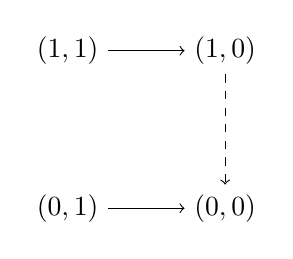
\begin{tikzpicture}[node distance=2cm, auto]
    \node (A) {$(1,1)$};
    \node (B) [right of=A] {$(1,0)$};
    \node (C) [below of=A] {$(0,1)$};
    \node (D) [right of=C] {$(0,0)$};
    \draw[->] (A) to node {} (B);
    \draw[->] (C) to node {} (D);
    \draw[->, dashed] (B) to node {} (D);
    \end{tikzpicture}\end{center}
  
  \label{fig:trivial-sm}
  \caption{A trivial state machine}
\end{figure}

To remedy this issue, we give a definition that gives a condition
under which it is safe to restrict the abstract IFC language
\ensuremath{L_\text{IFC}(\alpha,\Red{\lambda})}, such that non-interference is preserved.

\begin{definition}[Restricted IFC language]
  \label{def:restricted}
  For a family of predicates $\mathcal P$ (one for every reduction
  rule), we call
  \ensuremath{L_\text{IFC}^{\text{-}}(\mathcal{P},\alpha,\Red{\lambda})} a restricted IFC language
  if its definition is equivalent to the abstract language
  \ensuremath{L_\text{IFC}(\alpha,\Red{\lambda})}, with the following exception:
  The reduction rules are restricted
  by adding a predicate $P$ from $\mathcal P$ to the premise of
  all rule other than \textsc{I-noStep}.  Furthermore, the predicates $P$
  can depend only on the \textit{erased} configuration
  \ensuremath{\varepsilon_{\ifc{\Varid{l}}}(\ifc{c})}, where \ensuremath{\ifc{\Varid{l}}} is the label of the first task
  in the task list and \ensuremath{\ifc{c}} the full configuration.
\end{definition}

By the following theorem, the restricted IFC language with an
appropriate scheduling policy is non-interfering.

\begin{theorem}
  \label{thm:restricted}
  For any target language \ensuremath{\Red{\lambda}} and family of predicates
  $\mathcal{P}$, the IFC language \ensuremath{L_\text{IFC}^{\text{-}}(\mathcal{P},\textsc{RR},\Red{\lambda})}
  is TSNI.  Furthermore, the IFC language
  \ensuremath{L_\text{IFC}^{\text{-}}(\mathcal{P},\textsc{Seq},\Red{\lambda})} is TSNI.
\end{theorem}


\subsection{IFC language with a single heap}

We are now ready to make our single heap IFC language precise and
ensure its non-interference using the techniques presented.
First, we can construct the restricted language
\ensuremath{L_\text{IFC}^{\text{-}}(\mathcal{P}_\text{norefs},\alpha,\Red{\lambda_{\text{ML}}})}, where \ensuremath{\mathcal{P}_\text{norefs}} is
the family of always valid predicates, except for the ones for
\textsc{I-fork} and \textsc{I-send}, which we define as
\[ P = \text{\ensuremath{\ifc{\Varid{e}}} does not contain any address \ensuremath{\tar{a}}} \]
That is, we do not restrict any rules except for \textsc{I-fork}
and \textsc{I-send}.
Since $P$ only depends on \ensuremath{\ifc{\Varid{e}}}, which is part of the current
task and thus never erased w.r.t.\ the label of the first task,
this language satisfies non-interference by Theorem~\ref{thm:restricted}.

\begin{figure}
  
  \begin{mathpar}
    \inferrule[C-fork]
    {
      \text{\ensuremath{\ifc{\Varid{e}}} does not contain any \ensuremath{\tar{a}}}\\
      \ensuremath{\ifc{\Sigma}'\mathrel{=}\ifc{\Sigma}\left[\ifc{\Varid{i}}'\mapsto{}\epsilon\right]}\\
      \ensuremath{\ifc{\Varid{t}}_{1}\mathrel{=}\langle \ifc{E}\ifc{[}\ifc{\Varid{i}}'\ifc{]}\rangle^{\ifc{\Varid{i}}}_{\ifc{\Varid{l}}}}\\
      \ensuremath{\ifc{\Varid{t}}_\textrm{new}\mathrel{=}\langle \tar{_{\textrm{TI}}\lfloor}\ifc{\Varid{e}}\tar{\rfloor}\rangle^{\ifc{\Varid{i}}'}_{\ifc{\Varid{l}}}}\\
      \ensuremath{\textrm{fresh}\;(\ifc{\Varid{i}}')}
    }
    {\ensuremath{\ifc{\Sigma};\tar{\Sigma};\langle \ifc{E}\ifc{[}\mathbf{sandbox}\;\ifc{\Varid{e}}\ifc{]}_\ifc{I}\rangle^{\ifc{\Varid{i}}_{1}}_{\ifc{\Varid{l}}_{1}},\ldots\hookrightarrow\ifc{\Sigma}';\tar{\Sigma};\alpha_{{\tiny\mathrm{\Conid{F}}}}(\ifc{\Varid{t}}_{1},\ldots,\ifc{\Varid{t}}_\textrm{new})}}
    \and
    \inferrule[C-send]
    {
      \text{\ensuremath{\ifc{\Varid{e}}} does not contain any \ensuremath{\tar{a}}}\\
      \ensuremath{\ifc{\Varid{l}}\;\flows\;\ifc{\Varid{l}}'}\\
      \ensuremath{\ifc{\Sigma}\;(\ifc{\Varid{i}}')\mathrel{=}\ifc{\Theta}}\\
      \ensuremath{\ifc{\Sigma}'\mathrel{=}\ifc{\Sigma}\left[\ifc{\Varid{i}}'\mapsto{}(\ifc{\Varid{l}}',\ifc{\Varid{i}},\ifc{\Varid{e}}),\ifc{\Theta}\right]}
    }
    {\ensuremath{\ifc{\Sigma};\tar{\Sigma};\langle \ifc{E}\ifc{[}\mathbf{send}\;\ifc{\Varid{i}}'\;\ifc{\Varid{l}}'\;\ifc{\Varid{e}}\ifc{]}_\ifc{I}\rangle^{\ifc{\Varid{i}}}_{\ifc{\Varid{l}}},\ldots\rightarrow\ifc{\Sigma};\tar{\Sigma};\alpha_{{\tiny\mathrm{\text{step}}}}(\langle \langle\rangle\rangle^{\ifc{\Varid{i}}}_{\ifc{\Varid{l}}},\ldots)}}
  \end{mathpar}
  
  \caption{A selection of the reduction rules for \ensuremath{L_\text{IFC}^{\Red{\text{Heap}}}(\alpha)}.}
  \label{fig:concrete}
\end{figure}

The essential parts of the semantics for the concrete language
with a single heap,
which we call \ensuremath{L_\text{IFC}^{\Red{\text{Heap}}}(\alpha)},
are given in Figure~\ref{fig:concrete}.  Most rules are
straight-forward translations of the rules in Figures~\ref{fig:ifc}
and~\ref{fig:embedding} but for a single heap.  For conciseness, we
only show the interesting ones.
Now, we can show an isomorphism between this language and
\ensuremath{L_\text{IFC}^{\text{-}}(\mathcal{P}_\text{norefs},\alpha,\Red{\lambda_{\text{ML}}})}, which
(by Theorem~\ref{thm:iso-tsni} and~\ref{thm:iso-tini}) guarantees
non-interference for an appropriate scheduling policy \ensuremath{\alpha}.

\Red{Show the isomorphism.}


\section{Proofs}
\label{sec:proofs}

In this section we will prove all theorems we have stated so far.
We observe that the non-interference claims for the languages
\ensuremath{L_\text{IFC}(\textsc{Seq},\Red{\lambda})} and \ensuremath{L_\text{IFC}(\textsc{RR}_{{\tiny\mathrm{\cdot }}}(\cdot ),\Red{\lambda})}
in Theorems~\ref{thm:rr-tsni} and~\ref{thm:seq-tini} follow directly
from Theorems~\ref{thm:iso-tsni} and~\ref{thm:iso-tini},
respectively, about restricted IFC languages where the set
of predicates is the set of always valid predicates.

Before we proceed with the proof of Theorem~\ref{thm:iso-tsni},
we state a lemma we will use.

\begin{lemma}
  \label{lemma:rr-tsni-general}
  We consider, for any target language \ensuremath{\Red{\lambda}},
  the restricted IFC language \ensuremath{L_\text{IFC}^{\text{-}}(\mathcal{P},\alpha,\Red{\lambda})}
  (according to Definition~\ref{def:restricted}).
  Then,
  for any configurations \ensuremath{\ifc{c}_{1}}, \ensuremath{\ifc{c}_{1}'}, \ensuremath{\ifc{c}_{2}}, and label \ensuremath{\ifc{\Varid{l}}} where
  \begin{equation} \label{eq:tsni-lemma-lhs}
  \ensuremath{\ifc{c}_{1}} \approx_{\ensuremath{\ifc{\Varid{l}}}} \ensuremath{\ifc{c}_{2}}
  \qquad \text{and} \qquad
  \ensuremath{\ifc{c}_{1}} \ensuremath{\hookrightarrow} \ensuremath{\ifc{c}_{1}'}
  \end{equation}
  there exists a configuration \ensuremath{\ifc{c}_{2}'} such that
  \begin{equation} \label{eq:tsni-lemma-rhs}
  \ensuremath{\ifc{c}_{1}'} \approx_{\ensuremath{\ifc{\Varid{l}}}} \ensuremath{\ifc{c}_{2}'}
  \qquad \text{and} \qquad
  \ensuremath{\ifc{c}_{2}} \ensuremath{\hookrightarrow}^* \ensuremath{\ifc{c}_{2}'}
  \ \text{.}
  \end{equation}
\end{lemma}

\begin{proof}[Proof of Theorem~\ref{thm:iso-tsni}]
  We proof the theorem by induction on the length of the derivation sequence in~\eqref{eq:tsni-lhs}.
  The base case for derivations
  of length 0 is trivial, allowing
  us to simple chose $\ensuremath{\ifc{c}_{2}'\mathrel{=}\ifc{c}_{2}}$.  In the step case, we assume
  the theorem holds for derivation sequences of length up to $n$, and show that it also
  holds for those of length $n+1$.  We split the derivation sequence from~\eqref{eq:tsni-lhs} as follows:
  \[
  \ensuremath{\ifc{c}_{1}} \ensuremath{\hookrightarrow} \ensuremath{\ifc{c}_{1}''} \ensuremath{\hookrightarrow}^n \ensuremath{\ifc{c}_{1}'}
  \]
  for some configuration \ensuremath{\ifc{c}_{1}''}.  By Lemma~\ref{lemma:rr-tsni-general}, we get
  \ensuremath{\ifc{c}''} with
  \begin{equation} \label{eq:tsni-proof-1}
  \ensuremath{\ifc{c}_{1}''} \approx_{\ensuremath{\ifc{\Varid{l}}}} \ensuremath{\ifc{c}_{2}''}
  \qquad \text{and} \qquad
  \ensuremath{\ifc{c}_{2}} \ensuremath{\hookrightarrow}^* \ensuremath{\ifc{c}_{2}''}
  \end{equation}
  Applying the induction hypothesis to
  $\ensuremath{\ifc{c}_{1}''} \ensuremath{\hookrightarrow}^n \ensuremath{\ifc{c}_{1}'}$, we get \ensuremath{\ifc{c}_{2}'} with
  \begin{equation} \label{eq:tsni-proof-2}
  \ensuremath{\ifc{c}_{1}'} \approx_{\ensuremath{\ifc{\Varid{l}}}} \ensuremath{\ifc{c}_{2}'}
  \qquad \text{and} \qquad
  \ensuremath{\ifc{c}_{2}''} \ensuremath{\hookrightarrow}^* \ensuremath{\ifc{c}_{2}'}
  \end{equation}
  Stitching together the derivation sequences from~\eqref{eq:tsni-proof-1} and~\eqref{eq:tsni-proof-2} directly gives
  us the right-hand side of the implication in the TSNI
  definition~\eqref{eq:tsni-rhs}, which concludes the proof.
\end{proof}
\begin{proof}[Proof of Lemma~\ref{lemma:rr-tsni-general}]
  First, we observe there must be at least one task in \ensuremath{\ifc{c}_{1}}, otherwise
  it could not take a step.  Thus, \ensuremath{\ifc{c}_{1}} is of the form
  \ensuremath{\ifc{\Sigma}_{1};\ifc{\Varid{t}}_{1},\ifc{\Varid{ts}}_{1}}.  Consider two cases:
  \begin{itemize}
    \item $\ensuremath{\varepsilon_{\ifc{\Varid{l}}}(\ifc{\Varid{t}}_{1})}=\ensuremath{\bullet}$.
    By the definition of \ensuremath{\varepsilon_{\ifc{\Varid{l}}}}, we know that \ensuremath{\ifc{\Varid{l}}\;\flows\;\lcurr}
    where \ensuremath{\lcurr} is the label of \ensuremath{\ifc{\Varid{t}}_{1}}.
    In this case, we do not need to take a step for
    \ensuremath{\ifc{c}_{2}}, because \ensuremath{\ifc{c}_{2}'\mathrel{=}\ifc{c}_{2}} will already be \ensuremath{\ifc{\Varid{l}}}-equivalent to \ensuremath{\ifc{c}_{1}'}.
    To see that, note that the tasks \ensuremath{\ifc{\Varid{ts}}_{1}} in \ensuremath{\ifc{c}_{1}} are left in the
    same order and unmodified (the scheduling policy only
    modifies the first task). The task \ensuremath{\ifc{\Varid{t}}_{1}} either
    gets dropped (by \textsc{I-noStep}), or
    transforms into a task \ensuremath{\ifc{\Varid{t}}_{1}'} as well as potentially spawning a new
    task \ensuremath{\ifc{\Varid{t}}_{1}''}.  Since both \ensuremath{\ifc{\Varid{t}}_{1}'} and \ensuremath{\ifc{\Varid{t}}_{1}''} have a label that is
    at least as high as the label of \ensuremath{\ifc{\Varid{t}}_{1}} (can be seen
    by inspecting all reduction rules), they will get filtered
    by \ensuremath{\varepsilon_{\ifc{\Varid{l}}}} in \ensuremath{\ifc{c}_{1}'}.  Therefore, the \ensuremath{\ifc{\Varid{l}}} equivalence of the
    task list is guaranteed.
    Lets consider the possible changes to \ensuremath{\ifc{\Sigma}_{1}}:
    Only three reduction rules change \ensuremath{\ifc{\Sigma}_{1}},
    thus it suffices to consider these cases:
    \begin{description}
      \item[Case \textsc{I-send}]
      A new message triple with label \ensuremath{\ifc{\Varid{l}}'} gets added to the message
      queue of the receiving thread.  However, since \ensuremath{\lcurr\;\flows\;\ifc{\Varid{l}}'},
      the triple will get erased.
      \item[Case \textsc{I-recv} and \textsc{I-noRecv}]
      In this case, only the queue of
      task \ensuremath{\ifc{\Varid{t}}_{1}} can change, which gets erased.
    \end{description}
    This ensures that $\ensuremath{\ifc{c}_{1}'}\approx_{\ensuremath{\ifc{\Varid{l}}}}\ensuremath{\ifc{c}_{2}'}=\ensuremath{\ifc{c}_{2}}$.
%    \alphacondition{We need all scheduling policies to not change the order
%      of any tasks (except for the first one).  Newly spawned task can appear
%      anywhere in the list.}
    \item $\ensuremath{\varepsilon_{\ifc{\Varid{l}}}(\ifc{\Varid{t}}_{1})}\neq\ensuremath{\bullet}$.
    Here, there must be a corresponding
    task \ensuremath{\ifc{\Varid{t}}_{2}} in \ensuremath{\ifc{c}_{2}},
    such that \ensuremath{\ifc{\Varid{t}}_{1}\mathrel{=}\ifc{\Varid{t}}_{2}} (otherwise \ensuremath{\ifc{c}_{1}} and
    \ensuremath{\ifc{c}_{2}} could not be \ensuremath{\ifc{\Varid{l}}} equivalent).
    However, \ensuremath{\ifc{\Varid{t}}_{2}} might not be at the beginning of the task list yet, but
    all tasks occurring before it must get erased by \ensuremath{\varepsilon_{\ifc{\Varid{l}}}}.
    In \ensuremath{\ifc{c}_{2}}, we can first take some number of steps until \ensuremath{\ifc{\Varid{t}}_{2}} moves
    to the front of the list.
    This is the case regardless of any additional side conditions $P$ on
    rules, because for all of these tasks, it can either take an actual
    step, or it gets dropped by \textsc{I-noStep} (which is always
    possible, as there cannot be an additional side condition on this
    rule).  All tasks that didn't get dropped are still at a label
    that isn't below \ensuremath{\ifc{\Varid{l}}} and thus get erased.
    
%    \alphacondition{The scheduling policy must eventually let any task in
%      the task list evaluate.  In particular, it cannot get stuck when the
%      first task gets stuck, or keep executing a small number of tasks
%      exclusively forever (e.g. just execute the first task all the time
%      if it gets into an infinite loop).}
    
    Therefore, after \ensuremath{\ifc{c}_{2}} has potentially executed some number of steps
    to arrive at \ensuremath{\ifc{c}_{2}''}, we are now in the situation where $\ensuremath{\ifc{c}_{1}}\approx_{\ensuremath{\ifc{\Varid{l}}}}\ensuremath{\ifc{c}_{2}''}$, and the first tasks \ensuremath{\ifc{\Varid{t}}_{1}} and \ensuremath{\ifc{\Varid{t}}_{2}},
    respectively, don't get erased and are thus equivalent.
    The task \ensuremath{\ifc{\Varid{t}}_{2}} can now take exactly the same step as \ensuremath{\ifc{\Varid{t}}_{1}};  this
    is true even with arbitrary additional premises $P$ that follow
    the condition in Definition~\ref{def:npri}, since those
    predicates only depend on \ensuremath{\varepsilon_{\ifc{\Varid{l}}}(\ifc{c}_{1})}, which is equivalent
    to \ensuremath{\varepsilon_{\ifc{\Varid{l}}}(\ifc{c}_{2})}, and thus those predicates evaluate in the same way.
    Thus, we only
    need to argue that the potential differences in \ensuremath{\ifc{\Sigma}_{1}} and \ensuremath{\ifc{\Sigma}_{2}} cannot
    have an influence on the execution (and we know \ensuremath{\ifc{\Sigma}_{1}} and \ensuremath{\ifc{\Sigma}_{2}} are
    \ensuremath{\ifc{\Varid{l}}} equivalent).
    Again, only sending and receiving will depend on, or change \ensuremath{\ifc{\Sigma}},
    so we consider all these cases.
    \begin{description}
      \item[Case \textsc{I-send}]
      Here, the task \ensuremath{\ifc{\Varid{t}}_{2}} will send the same message to the same
      receiver queue. This
      queue is either completely erased, or it is \ensuremath{\ifc{\Varid{l}}} equivalent.  In both
      cases, \ensuremath{\ifc{\Varid{l}}} equivalence of \ensuremath{\ifc{\Sigma}_{1}'} and \ensuremath{\ifc{\Sigma}_{2}'} is preserved.
      \item[Case \textsc{I-recv} and \textsc{I-noRecv}]
      When the tasks are receiving a message, then by the reduction rules
      we know that they first filter the queue by the label
      \ensuremath{\lcurr} of \ensuremath{\ifc{\Varid{t}}_{1}}.  We
      also know that the queues are equivalent when filtered by the less
      restrictive label \ensuremath{\ifc{\Varid{l}}}, thus the messages received (or dropped) from the
      queue are equivalent.
    \end{description}
  \end{itemize}
\end{proof}


The proof of Theorem~\ref{thm:iso-tini} about TINI proceeds largely
in the same fashion as for Theorem~\ref{thm:iso-tsni} (TSNI), except that
some cases are simpler due to the fact termination is not an issue
(cf.~\tocite{} for a TINI proof of a similar system).

\section{The monadic interpretation}
\label{sec:monad}

In the previous sections, we have been primarily concerned with the
combination of operational semantics in order to automatically augment a
language with information flow control.  In this section, we present
a more abstract view of the situation, phrased in the language of monads
and monad transformers.  The key idea is that the computational effects
of the target language should be thought of as a \emph{monad transformer}
on top of the information flow control base monad.  Readers who are not
familiar with monads should feel free to skip this section.

Monads were originally proposed as a method for organizing computational
effects~\cite{Moggi:1991:NCM:116981.116984}.  One of the key questions
of interest was how to modularly build more complex computational
effects out of simpler ones.  One particular approach, the
\emph{incremental
approach}~\cite{Benton00monadsand,Liang95monadtransformers}, utilizes
monad transformers, which add an extra computation feature to a
pre-existing monad.  In the past, this approach has been criticized for
a number of failings, including the fact that the order in meaning of a
monad can depend on the order in which the monad transformers are
applied. The canonical example of this phenomenon is the
composition of the state monad and the error monad: depending on the
ordering of the two monad transformers, state is preserved or thrown away
upon an error.

These problems can be viewed as defects in a setting where we are
simply interested in combining effects.  However, in the setting of information
flow control, we are primarily interested in augmenting the
computational effects of a target language with information flow control
\emph{without} compromising non-interference.  When the base monad is
kept abstract (in the style of a restricted IO monad~\cite{Terei:2012:SH:2364506.2364524}),
there is an easy argument why any monad transformer must also preserve non-interference:
the monad transformer could have been implemented simply as a \emph{pure} interpreter, and
the pure interpreter is just another program like any other that may run on top of
a restricted IO monad.

Now, one shouldn't simply force an interpreter to be reimplemented on
top of a language supporting information flow control.  As suggested by
Filinski et al~\cite{Filinski:2010:MA:1707801.1706354}, we should use
pure implementations of computational effects to understand
computational effects when built into information flow languages: they
give a good hint what the operational rules should be.  This intuition
backed the development of Section~\ref{sec:retrofit}.  Furthermore,
developing the relationship between concrete semantics and abstract
semantics in Section~\ref{sec:concrete} relates to the question of monad
isomorphisms in the presence of data abstraction.  We leave the
investigation of this connection in more detail to future work.
\section{Real world languages}
\label{sec:real}

In the introduction, we stated that the original motivation behind
developing this embedding was in order to formally specify a
coarse-grained information flow control language for JavaScript.
%
In Section~\ref{sec:retrofit}, however, we used only a simplified
language as an example target language.
%
In this section, we consider the application of our embedding to
JavaScript and two other real world target languages, C and Haskell.
%
Our goal is to show the flexibility of the embedding in settings with
vastly different features and properties, as well as discuss the
semantic gap that must be overcome in some cases to apply our formalism
to other systems.
%
Two of the systems we describe have been implemented: the Haskell
system~\cite{lio} and the SWAPI~\tocite{} system; we leave the
implementation of the IFC system for C to future work.

\subsection{C}
\label{sec:real:c}
%
C programs are able to execute arbitrary (machine) code, access
arbitrary memory, and perform arbitrary syscalls.
%
Thus, the confinement of C programs must be imposed by the underlying OS
and hardware.
%
This isolation can be achieved using Dune's hardware protection
mechanisms~\cite{Belay:2012:DSU:2387880.2387913}, similar to a simpler
version of Wedge~\cite{Belay:2012:DSU:2387880.2387913,
Bittau:2008:WSA:1387589.1387611} with an information flow control
policy.
%
Using pages tables, a (trusted) IFC runtime could ensure that each task,
implemented as a lightweight process, can only access the memory it
allocates--tasks do not have access to any shared memory.
%
In addition, ring protection could be used to intercept syscalls performed by
a task and only permit those corresponding to our IFC language (e.g.,
\ensuremath{\mathbf{getLabel}}, \ensuremath{\mathbf{send}}).
%
Although other sandboxing mechanisms can be used in place of Dune, we
believe Dune's hardware protection mechanism would allow us to provide a 
concrete implementation that is more efficient and simpler to reason about.

In this setting, the combined language of Section~\ref{sec:retrofit}
can be interpreted in the following way: calling from the target
language to the IFC language corresponds to invoking a syscall.
%
Creating a new task with the \ensuremath{\mathbf{sandbox}} syscall is corresponds to
\emph{forking} a process.  Here, page tables limit what memory
a task can access: we can ensure there will be no memory (effectively
defining \ensuremath{\kappa\;(\tar{\Sigma})\mathrel{=}\tar{\Sigma}_{0}}, where \ensuremath{\tar{\Sigma}_{0}} is the set of pages necessary to bootstrap a
lightweight process.)
%
Similarly, control over page tables and protection bits allows us to
define a \ensuremath{\mathbf{send}} syscall that copies pages to our
(trusted) runtime queue; and, correspondingly, a \ensuremath{\mathbf{recv}} that copies
the pages from the runtime queue to the (untrusted) receiver.
%
Since C is not memory safe, conditions on these syscalls are
meaningless.


\subsection{Haskell}
\label{sec:real:hs}
In contrast with the C embedding which relies on hardware protection
mechanisms, a Haskell implementation can leverage Haskell's strong data
abstraction and static type system, monadic approach to effects, and
lightweight concurrency to implement the embedding in a more lightweight
manner.  We briefly describe one such system, LIO~\cite{lio}, which
implements IFC as a library.

LIO is implemented by defining a new monad, \text{\tt LIO}, which wraps Haskell's \text{\tt IO}
monad.
%
The purpose of this monad is twofold: it restricts the use of
arbitrary effects that would ordinarily be allowed by the \text{\tt IO} monad,
and it associates labels with tasks.
%
Computations in the \text{\tt LIO}
monad can be thought to be operating within the IFC system.
%
One important aspect of using \text{\tt IO} as the base for this
implementation is that it allows use of Haskell's efficient
implementation of threads, channels, etc. (e.g., in the concurrent
version of LIO, we use Haskell's \texttt{forkIO} to fork a lightweight
thread in the case of \ensuremath{\mathbf{sandbox}}~\cite{stefan:addressing-covert}), in
contrast to defining them in a completely pure fashion (as suggested
in Section~\ref{sec:monad}).

What is the interpretation of this system as per Section~\ref{sec:retrofit}?
%
Here, the \emph{pure subset} of Haskell is the target language, while
the monadic subset of Haskell in the \text{\tt LIO} monad is the IFC
language.
%
Crucially, the lack of unrestricted mutation in the pure fragment of
Haskell prevents direct communication between tasks, even when memory is
shared between them.\footnote{However, lazy evaluation can still produce
a covert channel.}

Since this IFC system is implemented as a library in Haskell,
implementation-wise, we must ensure that these languages are indeed the subsets of Haskell
we claim, i.e., while the concrete language is all of Haskell, we must
ensure that we can restrict programs to our subset of Haskell that
encodes the combined language.
%
To this end, \text{\tt LIO} relies on Haskell's strong data abstraction and type system
(as enforced by Safe Haskell~\cite{Terei:2012:SH:2364506.2364524}) to
ensure that arbitrary \text{\tt IO} actions cannot be lifted into
\text{\tt LIO}.
%
In other words, assuming \text{\tt LIO} is implemented correctly, programs
written in the \text{\tt LIO} monad cannot perform arbitrary \text{\tt IO} actions
without breaking abstraction.

We refer the interested reader to~\cite{lio,stefan:addressing-covert} for
additional details on the various implementations of this system.\footnote{It's worth noting that the proofs of non-interference we have given for asynchronous communication primitives are new and not in the original presentation of LIO.}


\subsection{JavaScript}
\label{sec:real:js}

JavaScript (JS), as specified by ECMAScript~\tocite{}, does not have any
built-in functionality for I/O. (Capabilities such as the ability to
mutate the DOM and read user input are APIs defined on top of the ECMAScript
specification.)
%
Consequently, and in contrast to our C and Haskell embeddings---for
which we must eliminate external effects---the embedding for JS is
trivial.

We describe SWAPI~\tocite{}, an implementation of this system for JavaScript.
%
The direct approach for implementing the embedded language \ensuremath{L_\text{IFC}(\textsc{RR},\Red{\lambda_{\text{JS}}})} is
by running multiple instances of the JS runtime, i.e., \ensuremath{\Red{\lambda_{\text{JS}}}}, in
separate OS-level threads.\footnote{
 The Firefox implementation of SWAPI also considers the case where
 tasks share the JavaScript runtime (and are cooperatively scheduled
 on the event-loop), but the heap and execution context of each task
 is disjoint. This is similar to the single-heap language of
 Section~\ref{sec:concrete}.  However, since the heap separation is
 provided by the browser the browser, we do not discuss this further.
 The interested reader is referred to~\tocite{} for more details.
}
%
In SWAPI, the IFC language functionality is implemented in the JS
runtime much like browser layout engines implement the DOM, and expose
the new functions, e.g., \text{\tt getElementById}, by attaching them to
the global JS object.
%
In turn, each task created with \ensuremath{\mathbf{sandbox}} is
executed in a separate thread, running a separate, \emph{fresh} instance of our
modified JS runtime.
%
Formally, \ensuremath{\mathbf{sandbox}} is defined with \ensuremath{\kappa\;(\tar{\Sigma})\mathrel{=}\tar{\Sigma}_{0}}, where \ensuremath{\tar{\Sigma}_{0}} is the global object corresponding to the standard
JS library (e.g., \ensuremath{\tar{\Sigma}_{0}} contains \texttt{Object}, \texttt{Array},
etc.).

Since this implementation approach relies on multiple runtimes of the
language, sending arbitrary objects between tasks can result in
unexpected behavior, e.g., when the object contains references.
%
As discussed in Section~\ref{sec:concrete}, we need to restrict \ensuremath{\mathbf{send}}
to expressions that can be marshalled as strings, i.e., structurally
clonable objects.
%
In our formalization, this amounts to restricting the IFC language rule
for \ensuremath{\mathbf{send}} such that only strings can be shared:
\newcommand{\str}{"string"}
\begin{mathpar}
\inferrule[JS-send]
{
\ensuremath{\ifc{\Varid{l}}\;\flows\;\ifc{\Varid{l}}'}\\
\ensuremath{\ifc{\Sigma}\;(\ifc{\Varid{i}}')\mathrel{=}\ifc{\Theta}}\\
\ensuremath{\ifc{\Sigma}'\mathrel{=}\ifc{\Sigma}\;[\mskip1.5mu \ifc{\Varid{i}}'\mapsto{}(\ifc{\Varid{l}}',\ifc{\Varid{i}},\ifc{\Varid{e}}'),\ifc{\Theta}\mskip1.5mu]}\\
\ensuremath{\ifc{\Varid{e}}\mathrel{=}\ifc{^{\textrm{IT}}\lceil}\tar{e}\ifc{\rceil}}\\
\ensuremath{\mathcal{E}_{\tar{\Sigma}}\left[\texttt{typeOf}(\tar{e})\texttt{ === \str}\right]\rightarrow\mathcal{E}_{\tar{\Sigma}}\left[\texttt{true}\right]}
}
{\ensuremath{\ifc{\Sigma};\langle \tar{\Sigma}, \ifc{E}\ifc{[}\mathbf{send}\;\ifc{\Varid{i}}'\;\ifc{\Varid{l}}'\;\ifc{\Varid{e}}\ifc{]}_\ifc{I}\rangle^{\ifc{\Varid{i}}}_{\ifc{\Varid{l}}},\ldots\hookrightarrow\ifc{\Sigma}';\alpha_{{\tiny\mathrm{\Sigma}}}(\langle \tar{\Sigma}, \ifc{E}\ifc{[}\langle\rangle\ifc{]}_\ifc{I}\rangle^{\ifc{\Varid{i}}}_{\ifc{\Varid{l}}},\ldots)}}
\end{mathpar}
We remark that this is similar to the existing
\texttt{postMessage} API used for iframe and Worker
communications~\cite{webworkers}.
%
Thus, the SWAPI implementation provides an IFC version of
\texttt{postMessage}, defined in terms of \ensuremath{\mathbf{send}}, that additionally
takes a label argument.

Unsurprisingly, our coarse-grained combined language approach has been
inspired by existing browser (security) architectures.
%
Browsers, for example, isolate pages of different origins by running
them in separate runtimes.
%
Similarly, they provide the Worker JS object~\cite{webworkers}, which allows
JavaScript to execute code in separate threads with separate JS
runtimes (and fresh global objects).
%
In both cases, code relies on the \texttt{postMessage} message-passing
API for communication, similar to our system.\footnote{
  The message-passing approach is, in part, due to ECMAScript's lack
  of well-defined semantics for concurrency.
  %
  Hence sharing and accessing objects such as the DOM across Worker
  threads is undefined.
}
%
As suggested by our formal semantics, SWAPI can directly leverage these
mechanisms to implement the semantics of \ensuremath{L_\text{IFC}(\textsc{RR},\Red{\lambda_{\text{JS}}})}
without modifying the JS runtime or intrusively changing the browser
layout engine.

However, a simple implementation of just associating a label with
Workers and browsing context (iframes and top-level pages) to enforce
IFC on the executing JavaScript is not sufficient, as APIs which
introduce extra computational effects must be manually made aware of information flow
control.
%
For example, the initial global object of a Worker contains the
\texttt{XMLHttpRequest} (XHR) object, while the global object of a
browsing context additionally contains the DOM.
%
In both cases, JS code can trivially leak information (e.g., to the
network with XHR or persistent storage using the DOM).
%
To address this, SWAPI additionally uses content security policy (CSP) and
(iframe) sandboxes~\tocite{} to restrict external effects according to
the label of a task (worker or browsing context).  Accomodating these
features lies outside the purview of our formalism.

%% \Red{
%% EZY:  This seems like useless detail about the SWAPI implementation
%% that is not relevant to this paper.
%% 
%% Of course, simply disallowing all external effects for all browsing
%% contexts would break most of the Web.
%% %
%% Hence SWAPI only enforces IFC, and thus restricts external effects,
%% when the JS code uses the new API.\footnote{
%%   Once a piece of code ``opts-in'' to use our IFC API, in addition to
%%   restricting external effects we interpose ``standard''
%%   \texttt{postMessage} communication to ensure that no information is
%%   leaked between contexts that have opted-in and those that have not.
%% }
%% %
%% Moreover, rather than disallowing all external effects, SWAPI allows
%% controlled network communication by leveraging the fact that web
%% pages already have an accompanying security policy: the same origin
%% policy.
%% %
%% Hence, for example, a Worker that has read data only sensitive to
%% \texttt{http://bank.ch} can communicate with this domain; only once
%% \texttt{http://aws.com} data is also included in the context will all
%% network requests be blocked.
%% %
%% Of course, this requires that we use a concrete label format to
%% express the policies; we refer the interested reader to~\tocite{} for
%% more details.}
\section{Extensions and Limitations}
\label{sec:extensions}

In this section we consider several extensions to our IFC system.
%
Specifically, we discuss how the specification language can be
extended to consider other IFC-aware features (e.g., fine-grained
labeled values), a static type system, or more complex scheduling
policies.
%
When considering these extensions we also highlight some limitations
of our approach.

\subsection{IFC language features}
\label{sec:extensions:labeled}

\paragraph{Labeled values}
\paragraph{Labeled references}
\paragraph{Labeled synchronization primitives}

\paragraph{Privileges}
Decentralized IFC extends IFC with the decentralized label model of
Myers and Liskov~\cite{myers:dlm} to allow for more general
applications, including systems consisting of mutually distrustful
parties.  In a decentralized system, a computation is executed with a
set of \emph{privileges}, which, when exercised, allow the computation
to declassify data (e.g., by lowering the current label).
%
Practical IFC systems
(e.g.,~\cite{Zeldovich:2006, lio,
Hritcu:2013:YIB:2497621.2498098, myers:jif}) rely on privileges to
implement many applications.
%
Since both the LIO and SWAPI implementations already support such features,
we believe that extending our calculus to consider privileges is
straight forward.
%
However, the challenge with such an extension lies in the precise
security guarantees that must be proved.
%
Addressing this problem is a natural direction for this work.

\paragraph{Clearance}
%
LIO, SWAPI, and Breeze additionally provide a discretionary access
control mechanism---called \emph{clearance}---at the language
level~\cite{Hritcu:2013:YIB:2497621.2498098, lio}; this mechanisms is
used to restrict a computation from accessing data (or communicating
with entities) above a specified label, the clearance.
%
For simplicity, we omitted clearance from our formalism.
%
We only remark that the mechanism generalizes beyond these IFC systems
in a straight forward manner and does not affect our definitions or
proofs in any meaningful way.


\subsection{Type safety}
\label{sec:extensions:types}

One important consideration for any new language feature is whether
or not it preserves type safety.  If implementations are allowed to
have undefined behavior when the system gets stuck, concerns of type
safety can be directly applicable to security.

In our presentation, we have demanded that implementations \emph{not}
have undefined behavior when getting stuck: in such situations, the
\textsc{I-noStep} rule applies, where the stuck thread should be dropped
from execution.  Our combined language will be not get stuck, even if
the target language could get stuck.  This sort of guarantee can be
achieved at a coarse granularity for languages like C by using hard
isolation.  However, for many other languages, this is too stringent a
requirement.

A possible way to relax this requirement is to drop the \textsc{I-noStep}
rule, and instead demand type-safety of the combined language.  This
depends on the type system of the target language, so it is difficult to
make any general statements about how one would go about doing this.  However,
there are few general remarks to be made:

\begin{itemize}
    \item In Matthews and Findlers original
        paper~\cite{Matthews:2007:OSM:1190216.1190220}, an emphasis was
        on using type boundaries to mediate between the type systems of
        the two languages, i.e. handling conversions of values from
        one language to the other.  These techniques are directly applicable here.

    \item In the case of mini-ML, type safety proceeds by a preservation theorem
        that refers to well-typed stores.  In our setting, there are now multiple
        stores, and expressions may move from being interpreted with one store
        to another (e.g. when an address is sent from one thread to
        another); a clear violation of type safety.  In this case, operations
        such as \textbf{send} have their typing rules require
        the expressions being sent be typeable in an arbitrary well-typed store,
        statically disallowing the sending of addresses, or any types which
        may contain addresses.  In practice, this may be further restricted to
        types which can be easily marshalled, e.g. strings.

    \item Similarly, the choice of $\kappa$ (from Section~\ref{sec:retrofit}) directly
        influences the difficulty of the type-safety proof for
        \textbf{fork} when the target language has a store.  When
        $\kappa$ is identity, most expressions can be allowed, since the store
        remains the same; if $\kappa$ drops the store, however, only closed expressions
        can be forked.
\end{itemize}

\subsection{Scheduling policies}
Our specification language is parametrized by a scheduling policy
\ensuremath{\alpha}, which maps a task list to a potentially different task list.
%
As previously discussed, the precise definition of \ensuremath{\alpha}
dictates whether the language is TSNI, TINI, or neither.
%
For simplicity we considered two popular policies \ensuremath{\textsc{RR}} and
\ensuremath{\textsc{Seq}} for which we showed TSNI and TINI, respectively.
%
However, our definitions allow for other scheduling policies that only
rely on the current task list.
%
For example, this allows us to implement the scheduler of~\tocite{}
that always schedules less sensitive threads first; this can be
employed to address external timing covert channels where an attacker
can measure the delay between output events.\footnote{
  When considering a label lattice that is not totally ordered, e.g.,
  DCLabels~\tocite{}, this scheduling policy is considerably more
  complex. See~\tocite{}.
}
%
More generally, we believe that deterministic schedulers that always
make ``low-progress,'' i.e., if a task whose label is not above the
current task's label will will eventually run, and do not decide which
low tasks to schedule according to data more sensitive than the tasks'
label, i.e., the scheduler does not schedule one public thread over
another according to sensitive data, to be safe.
%
We leave the proof of this claim to future work.
%

Despite allowing a number of practical schedulers to be expressed, our
scheduler parametrization is limited.
%
For instance, since \ensuremath{\alpha} is a map on task lists, schedulers that
rely on the global state \ensuremath{\ifc{\Sigma}} or previous task configurations cannot
be expressed.
%
Though, we do not believe this to be a fundamental limitation, our
current formalization cannot directly be applied to more-powerful, but
safe, scheduling policies, as considered in~\tocite{}.
%
More fundamentally, our definitions rely on deterministic relations,
and thus extending the system to consider non-deterministic schedulers
(or even non-deterministic target languages) is non-trivial.
%
For instance, this may potentially require the security condition to
consider \emph{low-determinism}, which states that a program is secure
only if \ensuremath{\Varid{l}}-equivalent results are deterministic~\tocite{}. %both andrei and steve's papers

\subsection{External effects}
\label{sec:extensions:external}
Our embedding assumes that the target language not have any
primitives that can external-world effects.
%
Indeed, as discussed in Section~\ref{sec:real}, part of the challenge
when considering real languages is precisely imposing this restriction
on the concrete implementation.
%
Yet, external effects are crucial when implementing more complex
real-world applications.
%
For example, code in our modified IFC browser must load resources or
perform XHR to be useful.

Like labeled references, features with external effects must be
modeled in the IFC language; we must reason about the precise security
implications of features that otherwise inherently leak data.
%
Previous approaches have modeled external effects by internalizing the
effects as writes/reads to labeled channels/references~\tocite{}.
%
An alternative approach is to model such effects as messages to/from
certain labeled tasks.
%
These ``special'' tasks are trusted with access to the unlabeled
primitives that can be used to perform the external effects; since the
interface to these tasks is already part of the IFC language, the
proof only requires showing that this task does not leak information.
%
This latter approach of wrapping unsafe primitives is, for example,
used in SWAPI to allow for controlled network communication.
%
By wrapping the default XHR object, for example, we can allow code
to communicate with hosts according to the task's current label.
\section{Related work}
\label{sec:related}

% Local Variables:
% TeX-master: "main.lhs.tex"
% TeX-command-default: "Make"
% End:



%Our paper follows a long tradition of papers on information flow
%control.  
Our information flow control system is closely related
to the coarse-grained information systems used in operating systems such
as Asbestos~\cite{efstathopoulos:asbestos}, 
HiStar~\cite{Zeldovich:2006}, and Flume~\cite{krohn:flume}, as well as language-based
\emph{floating-label IFC systems} such as LIO~\cite{lio},
and Breeze~\cite{Hritcu:2013:YIB:2497621.2498098}, where there is a
monotonically increased label
associated with threads of execution.
Our treatment of termination-sensitive and termination-insensitive interference
originates from Smith and Volpano~\cite{Smith:Volpano:MultiThreaded,Volpano:1997:ECF:794197.795081}.
%While this work often considers the interaction of information flow
%control with respect to various language features (e.g.,
%exceptions~\cite{Hritcu:2013:YIB:2497621.2498098}), none of these
%systems attempt to be generic in the choice of target language.

One information flow control technique designed to handle legacy code is
secure multi-execution (SME)~\cite{Devriese:2010}. It runs
multiple copies of the program, one per security level, where the semantics of
I/O interactions is altered. Authors often present
SME considering one specific programming
language~\cite{KULeuven-350547,Rafnson:2013}. However, Bielova
al.~\cite{Biel-etal-11-TR} uses a transition system to describe SME, where the
details of the underlying language is hidden.  Zanarini et
al.~\cite{ZanariniJR13} propose a novel semantics for programs based on
interaction trees~\cite{jacobs-tutorial}, which treats programs as black-boxes
about which nothing is known except what is inferred from their I/O interactions
with the environment. Similar to SME, our approach mediates I/O
operations; however, our approach only runs the program once.


One of the primary motivations behind this paper is constructing a practical
information flow control system for JavaScript.  Some of these systems attempt
to perform fine-grained information flow of
JavaScript~\cite{Hedin:2012,ConDOM,JSFlow}. While fine-grained information flow
control can result in less false alarms and target legacy code, it comes at the
cost of complexity (the system must accomodate the entirety of JavaScript's
semantics). Moreover, the runtime performance cost are sometimes too high, e.g.,
higher than 100\%!~\cite{JSFlow}.  Alternatively, coarse-grained approaches have
also been proposed for the web
scenario~\cite{Yip:2009:PBS,DeGroef:2012,conf/esorics/AkhaweLHSS13}. \Red{Different
from them, we rely on programming level abstraction to isolate
computations.}


%There are attempts to overcome this performance barrier by various means:
%Austin and Flanagan~\cite{Austin:Flanagan:PLAS09} handle this problem
%by using a \emph{sparse information labeling} scheme which reduces the
%cost of managing labels when they are not needed, while FlowFox~\cite{DeGroef:2012}
%uses an entirely different technique of \emph{secure multi-execution} to
%enforce non-interference. \Red{Probably more stuff here.}
%\todo{ds}{SME works for arbitrary language (kind of).}


The constructs in our IFC language, as well as the behavior of
inter-thread communication, is reminiscent of distributed systems
like Erlang~\cite{Armstrong03makingreliable}.  There is a close
correspondence: in distributed systems, isolation is required due to
physical constraints; in information flow control, isolation is
required to enforce noninterference.  Papagiannis et al.~\cite{Papagiannis_enforcinguser}
built an information flow control system on top of Erlang which is quite
similar to ours.  However, they do not use a floating label system (processes
can find out when sending a message failed due to a forbidden information flow),
and they include no security proofs.

There appears to be limited literature in general techniques for retrofitting
information flow control to arbitrary languages; however, one time-honored
technique is defining a fundamental calculus, for which other languages can be
desugared into.  Abadi et al.~\cite{abadi+:core} motivate their core calculus of
dependency by showing how various previous systems can be encoded in it; Tse and
Zdancewic~\cite{Tse:Zdancewic:ICFP04}, in turn, show how this calculus can be
encoded in System F via parametricity.  Broberg and Sands~\cite{Broberg:2010}
encodes several IFC systems into Paralocks.  However, this line of work is
primarily focused on static enforcements. 
%information flow control systems.

Our definition of isomorphism of information flow control languages in
Section~\ref{sec:concrete} is closely related to the idea of
\emph{bisimulation}~\cite{Milner:1989:CC:534666} and process calculi,
although as our system is deterministic, we do not use the theory in any
deep way.

It has long been observed that information flow control and monads are
closely related.  This observation has been used by Abadi et
al.~\cite{abadi+:core} to structure access to private data by protecting
it using a lattice of monads, one per security level. Russo et. al.~\cite{Russo+:Haskell08} extend this 
idea to languages with side-effects. Our system uses
monads in a conceptually different manner, where there is a single monad
representing the information flow control computational effects; this
is inline with the use of monads in other systems~\cite{Harrison05,lio,Devriese:2011}.
Devriese and Piessens~\cite{Devriese:2011} utilize monad
transformers as an essential component in their work.  However, their use
of monad transformers is to explain when extra constraints on a non-information
flow control aware base monad should be applied (i.e., during lifting).
Harrison and Hook~\cite{Harrison05} define a notion of \emph{atomic noninterference},
which is preserved through monad transformer application.  However, it is not
clear what is the relationship between this notion and traditional noninterference,
and their paper only proves a weaker property of no write down.

\cut{
\begin{itemize}
    \item Monads and IFC (Abadi~\cite{Abadi+:Core}, Tse~\cite{Tse:Zdancewic:ICFP04}, Harrison-Hook~\cite{Harrison05}, Crary~\cite{Crary:2005}, Devriese-Piessens~\cite{Devriese:2011})
    \item \Red{Operating systems approaches to IFC, which use coarse grained (Asbestos~\cite{efstathopoulos:asbestos}, HiStar~\cite{Zeldovich:2006})}
    \item \Red{Floating-label IFC systems, look at LIO paper (LIO~\cite{lio}, Breeze~\cite{Hritcu:2013:YIB:2497621.2498098})}
    \item JavaScript IFC related work, look at BrowBound. (ADSafe, xBook \Red{needs lookup})  Classify approaches into fine-grained (Hedin-Sabelfield~\cite{Hedin:2012}+JSFlow~\cite{JSFlow}, FlowFox~\cite{DeGroef:2012}, ConDOM~\cite{ConDOM}, Austin-Flanagan (sparse information labeling)~\cite{Austin:Flanagan:PLAS09}) or coarse-grained (BFlow~\cite{Yip:2009:PBS}, see Deian)
\item Secure multi-execution (FlowFox~\cite{DeGroef:2012}, Russo~\cite{Jaskelioff:SME})
\item Distributed programming languages (Cloud Haskell) plus IFC (Erlang (they check IFC when sending messages, no security proofs, assumes true isolation, not a floating labels)~\cite{Papagiannis_enforcinguser})
\end{itemize}


\Red{
Monads and IFC:

Basically, monads and IFC go together like toads and holes, or pigs and blankets, etc.  But the role the monad plays varies widely.  First, you have static systems (Abadi, Tse-Zdancewic), which utilize a lattice of monads: if a value is in a monad with a label that's too high, you're not allowed to unpeel it and look at the value inside.  Next, you have dynamic systems.  It seems pretty clear that making the IFC TCB be in a monad is a good idea, and the cluster of papers around LIO are all about that. Some of these papers talk about monad transformers: Devriese/Piessens focuses on how you might implement something like LIO by applying a monad transformer to some base monad to run the appropriate restrictions; Harrison/Hook do some more close to what we're doing, where they actually try to say something like "transformers do not interfere." But I can't tell if they're actually doing what we're doing, and their work has a number of unrelated technical restrictions.

In more detail:

Information Flow Enforcement in Monadic Libraries (Devriese/Piessens): Talks about how to use a monad transformer to take a non-IFC base monad and turn it into a IFC monad, namely the lifting operation should enforce extra constraints.  We take closely related ideas, and apply it to settings where there are not any monads.  Devriese/Piessens doesn't note the idea that untrusted monad transformers can be applied to add extra effects.

Achieving information flow security through monadic control of effects (Harrison/Hook): separation kernel is the basic idea behind our constructed (everything is partioned).  Notion of atomic noninterference between layers of effects, ``sufficient condition for atomic noninterference to be inherited through monad transformer application''.  But atomic noninterference is not proper noninterference as we've defined here! No proof of separation of kernels, instead prove weaker property no write down.

A Core Calculus of Dependency (Abadi et al): define a calculus, which calculi you want to prove IFC secure can be translated into.  It's a static system.  Why do they use monads?  Something about that
}


IFC for any language:

Gotta talk about secure multi-execution
}

%\cut{
\section{Conclusion}
\label{sec:conclusion}

We present a formal semantics which describes how to extend arbitrary languages
with language-based coarse-grained IFC. We provably show the security guarantees
TSNI and TINI non-interference, where the proof technique is parametrized on the
target language, and it is developed for two ubiquitous scheduling policies. In
addition, we provide conditions to securely refine our formal semantics to
consider optimizations required in practice. Finally, we describe extensions to
the core IFC language with more advanced concepts like labeled values, privileges,
and a notation of clearance, and therefore connecting it with existing
IFC implementations for Javascript, Haskell, and (in
less detail) proposing IFC for C.

With this work, we set a global framework which describes how ideas from
OS can be systematically applied in programming languages. 


% In this paper, we develop a general coarse-grained approach to IFC
% based on dividing a system into relatively course computational units
% and tracking only communication between these isolated units.
% We give formal semantics for the core coarse-grained
% information flow control language and show how a large class of target languages
% can be combined with it to achieve provable
% non-interference.
% We then give a proof technique for showing  non-interference
% of a concrete semantics for a potentially optimized IFC language
% by means of an isomorphism, and identify a class of IFC language restrictions
% that preserves non-interference.
% We briefly describe ways to enrich the core IFC language with
% more advanced concepts such as labeled values, privileges, or a
% notation of clearance and
% connect our formal semantics to real implementations of
% coarse-grained IFC systems for Javascript, Haskell, and
% (in less detail) enforcing IFC in C.
% Leaving more detailed presentation to later work,
% we informally relate our results to a monadic interpretation
% of IFC which guided our design.
% }


%{\frenchspacing\scriptsize
%\setlength{\bibsep}{2pt}
\bibliographystyle{abbrvnat}
\bibliography{local}

\end{document}

% Local Variables:
% TeX-master: "main.lhs.tex"
% TeX-command-default: "Make"
% End:
